

%% \documentclass[preprint,authoryear,12pt]{elsarticle}

%% Use the option review to obtain double line spacing
\documentclass[authoryear,preprint,review,12pt]{elsarticle}

%% Use the options 1p,twocolumn; 3p; 3p,twocolumn; 5p; or 5p,twocolumn
%% for a journal layout:
 %% \documentclass[final,authoryear,1p,times]{elsarticle}
%% \documentclass[final,authoryear,1p,times,twocolumn]{elsarticle}
%% \documentclass[final,authoryear,3p,times]{elsarticle}
%% \documentclass[final,authoryear,3p,times,twocolumn]{elsarticle}
%%\documentclass[final,authoryear,5p,times]{elsarticle}
%\documentclass[final,authoryear,5p,times,twocolumn]{elsarticle}


%% if you use PostScript figures in your article
%% use the graphics package for simple commands
%% \usepackage{graphics}
%% or use the graphicx package for more complicated commands
%%\usepackage{graphicx}
%% or use the epsfig package if you prefer to use the old commands
%% \usepackage{epsfig}

%% The amssymb package provides various useful mathematical symbols

%% The amsthm package provides extended theorem environments
%% \usepackage{amsthm}

%% The lineno packages adds line numbers. Start line numbering with
%% \begin{linenumbers}, end it with \end{linenumbers}. Or switch it on
%% for the whole article with \linenumbers after \end{frontmatter}.
\usepackage{lineno}

%% natbib.sty is loaded by default. However, natbib options can be
%% provided with \biboptions{...} comman. Following options are
%% valid:

%% round - round parentheses are used (default)
%% square - square brackets are used [option]
%% curly - curly braces are used {option}
%% angle - angle brackets are used <option>
%% semicolon - multiple citations separated by semi-colon (default)
%% colon - same as semicolon, an earlier confusion
%% comma - separated by comma
%% authoryear - selects author-year citations (default)
%% numbers- selects numerical citations
%% super - numerical citations as superscripts
%% sort - sorts multiple citations according to order in ref. list
%% sort&compress - like sort, but also compresses numerical citations
%% compress - compresses without sorting
%% longnamesfirst - makes first citation full author list
%%
%% \biboptions{longnamesfirst,comma}

\biboptions{round}

\usepackage{textcomp, fixltx2e}
\usepackage{fullpage, lscape}


\journal{Soil Biology and Biochemistry}
\usepackage{Sweave}
\begin{document}
\begin{frontmatter}

%% Title, authors and addresses

%% use the tnoteref command within \title for footnotes;
%% use the tnotetext command for the associated footnote;
%% use the fnref command within \author or \address for footnotes;
%% use the fntext command for the associated footnote;
%% use the corref command within \author for corresponding author footnotes;
%% use the cortext command for the associated footnote;
%% use the ead command for the email address,
%% and the form \ead[url] for the home page:
 %%
%% \title{Title\tnoteref{label1}}
%% \tnotetext[label1]{}
%% \author{Name\corref{cor1}\fnref{label2}}
%% \ead{email address}
%% \ead[url]{home page}
%% \fntext[label2]{}
%% \cortext[cor1]{}
%% \address{Address\fnref{label3}}
%% \fntext[label3]{}

\title{Controls of litter chemistry over early lignin decomposition in beech litter}

%% use optional labels to link authors explicitly to addresses:
 %% \author[label1,label2]{<author name>}
%% \address[label1]{<address>}
%% \address[label2]{<address>}

\author[1]{Lukas Kohl}
\author[1]{Wolfgang Wanek}
\author[2]{Katharina Keiblinger\fnref{boku}}
\author[1]{Sonja Leitner\fnref{boku}}
\author[1]{Maria Mooshammer}
\author[1]{Ieda H\"ammerle}
\author[1]{Lucia Fuchslueger}
%\author[1]{Alexander Frank}
\author[1]{J\"org Schnecker}
\author[2]{Sophie Zechmeister-Boltenstern\fnref{boku}}
\author[1]{Andreas Richter}
%%%>>>>corresponding author?!

\address[1]{Department of Chemical Ecology and Ecosystem Research, University of Vienna, Althanstra\ss e 14, A-1090 Vienna, Austria}
\address[2]{Federal Research and Training Centre for Forests, Natural Hazards and Landscape, Department of Soil Biology, Seckendorff-Gudent-Weg 8, A-1131 Vienna, Austria}
\fntext[boku]{Current adress: Institute for Soil Science, University of Natural Resources and Life Sciences, Peter Jordan-Stra\ss e 82, A-1190, Vienna, Austria}

\begin{abstract}
Lignin is considered the most recalcitrant component of plant litter, accumulated during early decomposition and degraded only during late decomposition stages when its concentration limits litter decomposition rates. A recent study based on the more specific methods challenges this concept, reporting highest lignin decomposition rates during early litter decomposition. Until now, no further studies exploring early lignin decomposition were published, and its potential controls remain unknown.

We follow lignin and carbohydrate decomposition during early litter decay with analytical pyrolysis in a climate-chamber decomposition experiment, focusing on resource control over microbial carbon substrate preferences. Beech litter with different C:N:P stoichiometry but identical initial microbial communities was incubated to identify the control of litter chemistry on the developing microbial community and its decomposition activity. 

During the first 6 month fundamental differences in lignin degrading activities were found between sites. Lignin discrimination in litter decomposition ranges from insignificant amounts of lignin decomposed to lignin decomposition at the same rate bulk litter, leading to different niveaus of lignin accumulation. Between 6 and 15 month, no lignin discrimination was found, but different lignin contents aquired earlier reminded.

[results]
%Neither nitrogen nor labile carbon availability could be identified as a control over lignin decomposition. However, amounts of lignin decomposed were correlated to the buildup of resource to decomposer C:N and C:P imbalances.

\end{abstract}
\begin{keyword}
%% keywords here, in the form:
 litter decomposition \sep lignin \sep analytical pyrolysis \sep Pyr-GC/MS

%% MSC codes here, in the form: \MSC code \sep code
%% or \MSC[2008] code \sep code (2000 is the default)
\end{keyword}
\end{frontmatter}

\linenumbers
\section{Introduction}
Plant litter biomass is dominated by macromolecular compounds. Together, lignin, carbohydrate and protein polymers make up xx\% of litter dry mass, while leach-able substances in litter account for only xx \%. 

Litter decomposition models [lit] follow the concept that macromolecules in litter form three independent carbon pools of increasing recalcitrance attributed to (1) soluble compounds, (2) cellulose and hemi-celluloses and (3) lignin. During decomposition, soluble compounds are most accessible to microbes and consumed first, followed by carbohydrates (i.e. cellulose). Lignin can be decomposed only by specialists and is not degraded until accumulated to a certain, critical level when it inhibits the degradation of less recalcitrant compounds \citep{Berg1980, Couteaux1995, Moorhead2006}.\footnote{more lit.} Most common methods to quantify these carbon pools gravimatrically determine cellulose, hemi-celluloses and lignin contents after sequential extractions with selective solvents. These methods were repeatedly criticize as unspecific for lignin determination \citep{Hatfield2005}. When analyzed with alternative methods (NMR, CuO-oxidation, Pyrolysis-GC/MS), extracted lignin fractions contain many other than the proclaimed substances. (i.e. \cite{Preston1997} \footnote{[lit CuO], lit[Pyr]}. 

Recent studies based on specific methods to determine litter lignin content (CuO - oxidation, Pyrolysis-GC/MS, NMR) question the assumed intrinsic recalcitrance of lignin. Experiments using isotope labeling used to calculate mean residence times for lignin in soils and litter/soil mixtures in both laboratory and outdoor incubation reported lignin residence times no longer than that of other carbon compounds or bulk SOM \citep{Thevenot2010a, Bol2009}\footnote{more lit?}.

For leaf litter, lignin depletion during early decomposition and decreasing lignin decomposition rates were recently by \cite{Klotzbucher2011}. Based on their results, the authors proposed a new concept for lignin degradation in which fastest lignin degradation occurs during early litter decomposition. Lignin decomposition during late decomposition is limited by (dissolved organic) carbon availability, a pulsed input of labile carbon (during litterfall or experimental manipulations like drying and rewetting) causes higher lignin degradation rates for a limited time period. The authors also suggest, that lignin decomposition is hampered in late decomposition stage, when labile (soluble) carbon source are limited. %This concept is supported by results from decomposition experiments with \emph{Arabidopsis thaliana} mutants. Lignin decomposition was completely inhibited in a low-cellolose mutant \citep{Talbot2011}.

\cite{Klotzbucher2011} do not elaborate the of stoecheometric constrains on lignin decomposition. In isolated lignin fractions from fresh beech litter, N contents twice as high as bulk litter were found \footnote{cit}. It was argued that, while yielding little C and energy, lignin decomposition makes occluded cell wall protein accessable to decomposers, and lignin decompostion is driven not by carbon but by nitrogen demand ("Nitrogen mining theory", \cite{Craine2007}). 

Nitrogen fertilization experiments on litter and soils indicate a that litter N contents are important controls of lignin degradation: N addition increases mass loss rates in low-lignin litter while slowing down decomposition in lignin-rich litter \citep{Knorr2005}. High nitrogen levels were reported to inhibit lignolytic enzyme in forest soils\citep{Sinsabaugh2010}. Cellulose triggered higher priming effect in fertilized than in unfertilized soils indicating that the mineralization of recalcitrant C is controlled by an interaction of labile C and N availability \citep{Fontaine2011}.

N fertilization has different effects on litter decomposition than different nutrient levels in litter, as leaf litter N is stored in protein and lignin structures and not directly availeable to microorganisms. N-fertilization experiments can simulate increased N-deposition rates. To simulate variations litter C:N ratios, our approach is preferable, because potential variations in litter N content occur in complex substrates.

In this study we analyze samples from climate-chamber incubated beech litter varying in N and P content with pyrolysis-GC/MS (pyr-GC/MS). The experiment was designed to study the effect of resource stroichiometry on microbial decomposition, exclude decomposing fauna and keep climatic conditions constant.

We test several proposed mechanisms, by which lignin degradation is affected by litter chemistry:

(1) High lignin contents inhibit the degradation of other carbon sources, and trigger lignin decomposition \citep{Berg1980}.

(2) Lignin degradation is inhibited, when the availability of cofactors for oxidative enzymes (mainly Mn) is low \footnote{cit}.

(3) Lignin degradation is directed to degrade N, therefore less lignin is decomposed in litter with narrow C:N ratios where more lignin is available \citep{Craine2007}.

-(4) The availability of dissolved carbon limits lignin decomposition, and lignin decomposition is inhibited when DOC content becomes rate limiting (and therefore correlated to) carbon respiration rates\citep{Klotzbucher2011}.
% [Elevated N deposition and elevated soil N content increase litter N contents, while a recent meta-study hints that elevated atmospheric CO$_{2}$ concentrations cause wider litter C:N ratios \citep{Luo2006}. Therefore it is important to assess the impact of shifts in litter C:N ratio on decomposition processes and the chemical nature of the resulting organic matter to predict feedback mechanisms of anthropogenic alterations of global carbon and nitrogen cycles. While predictions of changes in mass loss rates under alternated litter C:N ratios are abound [lit.], no studies on changes in the quality of litter biomass during and after decomposition or of the dynamics of accumulation/depletion of fragments of the litter biomass during decomposition exist yet.]

%Also, interdependance of these pools seems much higher than expected. Lignified cellulose and protein is not accessable without degrading lignin... Ligin fractions extracted from (fresh) beech litter have beed demonstrated to have a very narrow C:N ratio if compared to bulk litter, nonligneous cell walls or soluble matter. It is assumed, that proteins are covalently bound to lignin polymers during polymerization. For litter decomposing microbia this implies that degrading lignin increases nitrogen availability, while degrading non-lignified carbohydrates yields more metabolic energy, but no additional nitrogen. In an incubation eperiment with a litter/soil mixture, N addition stimulated carbon mineralization during the first weeks of incubation but slowed it down duringThe after with ratios after climate chamber incubation for up to 15 month. late decomposition.

%In temperate forests, litter decomposition is generally considered nitrogen limited (lit).
%several experiments report retention times for lignin in soil [not much higher than other soil components].

%Several recent studies apply analytical pyrolysis (Pyr-GC/MS) to characterize complex natural organic polymers like soil organic matter (SOM, \cite{Vancampenhout2010}[more lit here]).
%Only a limited number of pyrolysis studies comparing different decomposition levels have been done.
%Pyrolysis-based decomposition studies usually focus on the woody material \citep{Vinciguerra2007} or soil/litter mixtures [lit! - z.b. gleixner ca.1999]. Microbial decomposition of straw was followed by Pyr-GC/MS by [lit] We found only one study analyzing different stages of litter decomposition with analytical pyrolysis \citep{Franchini2002} and one recent study using a related technique (thermally assisted hydrolysis and methylation in \citep{Snajdr2011}.

%\cite{Kuder1998}

%European beech (\emph{Fagus silvaticus} L.) is the dominant forest building tree species in central europe.

%Extensive data on litter chemistry and and decomposition process rates are available for this samples from previously publications \citep{Mooshammer2011, Wanek2010, Leitner2011}.

%We hypothesize that

%(1) While (non-lignified) carbohydrates are easier degraded than lignin and the resulting sugar monomers yield more energy, lignin degradation improves to accessibility of nitrogen (``lignin mining'', \cite{Craine2007}). More lignin is decomposed when nitrogen availability is low, and high nitrogen availability inhibits lignin degradation.

%(2) Lignin degradation is inhibited when labile (dissolved) carbon availability is low and decomposition is energy limited (as proposed by \cite{Klotzbucher2011}).

%(3) Lignin decomposition yields less energy than carbohydrate decomposition, therefore carbon loss and decomposition process rates are lower in litter that decomposes more lignin.

 %Their accumulation and/or depletion during decomposition was extensively studied, nevertheless recent studies based on new methods to measure lignin content challange traditional models.

 % Decomposition conditions control whether assimilated carbon is released immideately or sequestered to soil organic matter. Decomposition processes also control the quality of the resulting organic matter and therefore soil carbon recalcitrance.

 %\cite{Prescott2010} suggests the amount of remaining biomass more important than the decomposition speed. We suggest, the chemical nature of this remaining biomass might be a factor too. we should study the influences of environmental parametres on the chemical conposition of the remaining biomass.

 % but using methods based on detergent extraction no regarded unspecific.

 %Large scale experiments (lit!) conducted during the last years collected detailed data on chemical and ecological controls predict dry mass loss during litter decomposition. Nevertheless, understanding of chamical transformations in litter loss is still limited, as most studies limit their analysis of high molecular weight compounds to detergent extraction based methods (Klason Lignin, ... - lit).


 %\cite{Snajdr2011a} used THM (a pyrolysis-related method) in a litterbag expiriment, but limits analysis to determining lignin:carbohydrate ratios.

 %These studies often explain biomarkers found in SOM by their occurance in a plant polymers and propose a decendence from thos biomarkers \citep{Schellekens2009b}, some of them also analyze local vegetation for comparison.

\section{Material and methods}
\subsection{Litter decomposition experiment}
A detailed description of our litter decomposition experiment was published in \cite{Wanek2010}. Briefly, beech litter was collected at four different sites in Austria (Achenkirch (AK), Klausenleopoldsdorf(KL), Ossiach(OS), and Schottenwald(SW); refered to as litter types) in October 2008. Litter was cut to pieces of approximately 0.25cm$^2$, homogenized, sterilized twice by gamma\footnote{greek gamma here} radiation (35 kGy, 7 days between irradiations) and inoculated (1.5\% w/w) with a mixture of litter and soil to assure that all litter types share the same initial microbial community. From each type, four samples of litter were taken after inoculation and stored dried at room temperature. Samples of 60g litter (fresh weight) were incubated at 15 \textdegree C and 60\% water content in mesocosms for a duration between 2 weeks to 15 month. For each litter type 5 replicas were removed and analyzed after 14, 97, 181 and 475 days.

Litter chemistry as analyzed 14 days after incubation is listed in table \ref{initstoech}. C:N ratios between 1:41 and 1:58 and C:P ratios between 1:700 and 1:1300 were found, N:P ratios ranged between 1:15 and 1:30. No significant changes occurred during litter incubation except a slight decrease of the C:N ratio (1:41.8 to 1:37.4) found in the most active litter type (SW) after 15 month. Fe content were more than twice as high for OS (approx. 450 ppm) than for other litter types (approx. 200 ppm). Litter Mn also was highly variable between litter types, ranging between 170 and 2130 ppm. Changes of micro-nutrient concentrations during litter incubation were significant, but in all cases \textless 15\% of the initial concentration.

\subsection{Bulk litter, extractable, and microbial biomass nutrient content}
To calculate litter mass loss, litter dry mass content was measurement in 5 g litter (fresh weight) after 48 h at 80 \textdegree C. Dried litter was ball-milled for further chemical analysis. Litter C and N content were determined using an elemental analyzer (Leco CN2000, Leco Corp., St. Joseph, MI, USA). Litter phosphorus content was measured with ICP-AES (Vista-Pro, Varian, Darmstadt, Germany) after acid digestion \cite{Henschler1988}).

To determine soluble C, N, and P contents, 1.8g litter (fresh weight) were extracted with 50 ml 0.5M K\textsubscript{2}SO\textsubscript{4}. Samples were shaken on a reciprocal shaker with the extractant for 30 minutes, filtered with ash-free filters and frozen at -20 \textdegree C until analysis. To quantify microbial biomass C, N and P pools, sample were extracted under the same conditions after chloroform fumigation. Microbial biomass was determined as the difference between fumigated and non-fumigated extractions \citep{Schinner1996}. C and N concentration in extracts were determined with a TOC/TN analyzer (TOC-VCPH and TNM, Schimadzu), Phosphorous was determined photometrically.\footnote{lit!!}

Substrate to consumer stoichiometric imbalances \emph{X:Y$_{inbal}$} were calculated as
\begin{equation}
 X:Y_{inbal}=\frac{X:Y_{litter}}{X:Y_{microbial}} \label{eq:resp.acc}
\end{equation}
where \emph{X} and \emph{Y} stand for one of the elements C, N, or P.

\subsection{Microbial Respiration}
Respiration was monitored weekly during the entire incubation in mesocosms removed after 6 month and on the last incubation day for all mesocosms using an infrared gas analyzer (IRGA, EGM4 with SRC1, PPSystems, USA). CO2 concentration was measured over 70 seconds and increase per second was calculated based on initial dry mass. Measurements of ambient air were performed before and after each measurement to assess possible leaks or base-line drifts IRGA. %Measurements were conducted using the following settings: volume of the chamber 1551 cm³, area of the chamber 115 cm², linear measurement, at 15\textdegree.
Accumulated respiration after 6 month was calculated assuming linear transition between measurements, accumulated respiration after 15 month was estimated from respiration rates after 181 and 475 days.
%as stated in equation \ref{eq:resp.acc}, where \emph{Resp\textsubscript{acc}} stands for the accumulated respiration, \emph{Resp\textsubscript{n}} and \emph{t\textsubscript{n}} for the actual respiration at and the decomposition time until time point \emph{n}.

% \begin{equation}
% Resp_{acc}(t_{n})=\sum_{i=0}^n (Resp(t_{i})+Resp(t_{i+1}))*(t_{i+1}-t_{i})/2
% \label{eq:resp.acc}
% \end{equation}


\subsection{Enzyme activities}

Measurements of potential exo-enzyme activities for cellulases, peroxidases and phenoloxidase were described by \cite{Leitner2011}. Activities were determined with a series of micro-plate assays based on the hydrolysis of 4-methyl-$\beta$-D-cellobioside (cellulase) and L-3,4-di\-hydroxy\-phenyl\-alanin (oxidative enzymes). Products of enzyme catalyzed reactions were detected photometrically (oxidative enzymes) or flourometrically (cellulase) \citep{Marx2001, Sinsabaugh1999, Kaiser2010b}.

\subsection{Pyrolysis-GC/MS}
Pyrolysis-GC/MS was performed with a Pyroprobe 5250 pyrolysis system (CDS Analytical) coupled to a Thermo Trace gas chromatograph and a DSQ II MS detector (both Thermo Scientific) equipped with a carbowax colomn (Supelcowax 10, Sigma-Aldrich).

Litter analyzed was sampled immediately after inoculation and after 3, 6, and 15 month incubation. 2-300 \textmu g dried and finely ball-milled litter were heated to 600\textdegree C for 10 seconds in helium atmosphere. GC oven temperature was constant at 50 \textdegree C for 2 minutes, followed by an increase of 7\textdegree C/min to a final temperature of 260 \textdegree C, which was held for 15 minutes. The MS detector was set for electron ionization at 70 EV cycling between m/z 20 and 300.\footnote{maybe cite other paper for method?}

Peaks were assignment was based on NiSt 05 MS library after comparison with reference material measured. 128 peaks were identified and selected for integration due to their hight abundance or diagnostic value, including 28 lignin and 45 carbohydrate derrived substances. For each peak between one and four dominant mass fragments selected for high abundance and specificity were integrated and converted to TIC peak areas by a multiplication with a MS response coefficient \citep{Schellekens2009, Kuder1998}. For principal component analysis, unconverted areas were used. Peak areas are stated as \% of the sum of all integrated peaks of a sample.

 % TIC peak areas are (1) less specific as areas of specific MS fragments and (2) integration was not possible for all peaks a/o all samples. Therefore a MS response factor Rf was calculated for each detected substance:
 %\begin{equation}
 %$Rf = median \left(\frac{TIC peak area}{specific MS fragment peak area}\right)$
 %\end{equation}

 %Peak areas were multiplied by Rf before addition to calculate percentages of TIC area without loosing the specifity of integrating single m/z traces.

 % However, during interpretation, we found little difference between direct sums of the integrated fragments and sums of corrected areas, indicating little sensitivity for exact

Relative peak areas are different from weight\%, but allow tracing of accumulation/depletion of substance classes during decomposition \citep{Schellekens2009}.

We use the terms "accumulation" and depletion to refer to changes in litter composition and "degradation" to refer to the amount of lignin and carbohydrates decomposed.

A lignin to carbohydrates index was calculated to measure the ratio between these two substance classes without influences of changes in the abundance of other compounds
\begin{equation}
 LCI=\frac{Lignin}{Lignin + Carbohydrates}
\end{equation}

Accounting for carbon loss, we estimate \% lignin and cellulose degraded during decomposition according to equation \ref{eq:closscorr}, where \emph{$TIC_{init}$} and \emph{$TIC_{act}$} stand for initial and actual \%TIC area of lignin or cellulose pyrolysis products, \emph{$C_{init}$} for the initial amount of C and \emph{$R_{acc}$} for the accumulated CO$_2$-C respired by a mesocosm.
\begin{equation}
 \%_{loss} = 100\cdot\frac{TIC_{init}-TIC_{act}}{TIC_{init}}\cdot\frac{\left ( 1-R_{acc}\right ) }{C_{init}}
 \label{eq:closscorr}
\end{equation}

We provide \% of initial lignin and carbohydrate pools decomposed, \% decomposed per \% litter carbon mineralized and the ratio between the twodecomposition rates.

\subsection{Statistical analysis}
All statistical analyses were performed with the software and statistical computing environment R using the package ``vegan'' \citep{Oksanen2011}. If not mentioned otherwise, results were considered significant when p \textless 0.05. Due to the frequent of variance inhomogenities Welch anova and paired Welch's t-tests with Bonferroni corrected p limits were used. Principal component analysis was performed using vegan function ``rda'' scaling variables. All correlations refer to Pearson correlations. We calculated correlations between depletion and degradation rates found in this study with litter chemistry parametres and process data reported by \cite{Mooshammer2011} and \cite{Leitner2011}.

\section{Results}

\subsection{Mass loss, respiration and extractable organic carbon}

Litter mass loss was not significant after 2 weeks and 3 month, significant for 2 litter types after 6 month. After 15 month, litter mass loss was significant for all litter types, and strongly correlated to litter N content (R=0.794, p=***). Detailed results were reported by \citep{Mooshammer2011}. After 15 month, between 5 and 12\% of the initial dry mass was lost. This is less than reported in litter decomposition studies on other species, but in a similar range as recently reported for beech litter from an in-situ litterbag-study \citep{Kalbitz2006} .

Highest respiration rates were measured after 14 days incubation (150-350 \textmu g CO\textsubscript{2}-C d-1 g-1 litter-C), dropped to rates between between 75 and 100 \textmu g CO\textsubscript{2}-C d-1 g-1 litter-C after 97 days. After 181 and 375 days, respiration rates for AK and OS further decreased, while SW and KL show a second maximal respiration after 181 days. %Respiration was correlated to litter N content after 2 weeks, 6 and 15 month(R\textgreater 0.70 in all cases, all p \textless  0.001), but not after 3 month. All harvests combined were weakly correlated to litter N content (R=0.416, p \textless  0.001).
%Accumulated respiration was correlated to litter mass loss for all harvest with significant mass loss when means per litter type and harvest were compared (n=6).

Soluble organic carbon content decreased between the first three harvests (14 to 181 days), to strongly increase after 475 days (0.1 to 0.7 mg C g $^{-1}$ d.w. were found after 14, 97 and 181 days, and increased to amounts between 1.5 and 4 mg/g after 375 days. After 14 and 97 days, the highest C content was found in SW litter followed by AK (see fig. \ref{fig:doc}. DOC content was loosely correlated to litter N content after 14 (R=0.69, p\textless  0.001) and 97 days (R = 0.65, p =\textless  0.01), they were strictly correlated after 181 days (R = 0.85, p=\textless  0.001) and 375 days (R=0.90, p=\textless  0.001).

%\begin{figure*}[t]
%\vspace*{2mm}
%\begin{center}
%\setkeys{Gin}{width=0.5\textwidth}
%<<doc, echo=F, results=hide, fig=T, height=7, width=7>>=
%timeseries(alldata$DOC/1000, alldata$days, alldata$Litter, pch=pch, pt.bg=colscale,  xlab="Incubation (days)", ylab="mg C g-1 d.w.", main="Extractable carbon", lwd=2)
%legend("bottomright", pt.bg=colscale, pch=pch, typlev, lty=1, lwd=2)
%@
%\end{center}
%\caption{Extractable organic carbon. Error bars indicate standard errors (n=5).}
%\label{fig:doc}
%\end{figure*}


\subsection{Microbial biomass abundance and stoichiometry}

Microbial biomass contents ranged from 0.5 to 6 mg C, 0.05 to 5.5mg N and 0.05 to 3.5 mg P per g litter (d.w.). In KL and OS biomass buildup reaches a plateau after 3 month, AK and SW show further growth reaching a maximum of microbial C and N contents after 6 month (AK also for P). Microbial C:N ratios measured range between 1:6 and 1:18, C:P ratios between 1:8 abd 1:35, and N:P ratios between 1:0.5 and 1:3.5. Microbial C:N ratios (Fig. \ref{fig:mb}).


Litter microbial biomass is homeostatic during the first 6 month (no or marginally negative correlation between microbial stoichiometry and litter stoichiometry) \citep{Mooshammer2011}, but not after 15 month, when all three ratios show correlations (R 0.53 - 0.64, all p \textless 0.002, H\textsubscript{C:N}=2.01, H\textsubscript{C:P}=1.68, H\textsubscript{N:P}=2.29). Microbial C:N ratios are tighly constrained after 3 (1:14.5 - 1:18.2) and 6 month (1:6.9 - 1:9.0), but significantly different between the two time points. C:P and N:P ratios are less constrained, with the highest variance between litter from different sites after 3 month incubation (Fig. \ref{fig:mb}).

\subsubsection{Potential enzyme activities}
Absolute potential enzyme activities were correlated to litter N, respiration and other other decomposition processes (all R \textgreater  0.8, p \textless 0.001). For all enzymes and at all time points, SW showed the highest and AK the lowest activity. Cellulase was below detecten limit after 14 days, oxidatitve enzymes after 15 month. Cellulases activity is highest after 3 month and decreases between 97 and 181 days. Peroxidase and Peroxidase activities reach their maximum after 181 (fig. \ref{fig:enz}). After between 6 and 15 month, cellulase activity strongly increased. After 475 days, the activity of oxidative enzymes was below the detection limit [data not shown]

The ratio between the potential activities of cellulases and oxidative enzymes was lowest for AK at all time points. Microbial communities in AK litter invest more energy and nitrogen into degrading lignin and less into degrading carbohydrates than other litter types. (fig. \ref{fig:enz})

\subsection{Pyrolysis-GC/MS and Lignin content}
%Lignin contents determined by ADF extraction show initial lignin contents between 15 and 21 \% d.w.. After 3 month, lignin contents rise to levels above 30\% d.w. in two sites, an increase that can not be explained by passive accumulation \cite{Leitner2011}.

Litter pyrolysis products and different sites are reported in detail elsewhere (Kohl, in preparation). We found only minor changes during pyrograms during decomposition, differences between sites were were small but well preserved during decomposition. The high similarity allowed tracind small changes in lignin and carbohydrate abundance during decomposition. % A PCA performed on relative peak areas of 128 peaks shows that samples cluster according to litter types, with no constistent seperation between different harvests. \ref{fig:pca1}. %118 (94.5\%) [!check nr!] of the peaks integrated show significant differences in relative peak areas between different litter types before incubation.

When measured by pyr-GC/MS, lignin derrived compounds make up between 29 and 31 \%TIC in the initial litter, with an increase of up to 3 \%TIC over the first 3 month. Carbohydrate derrived pyrolysis products account for 26 to 29 \%TIC in initial litter and decrease by up to 2.6 \% during litter decomposition. Carbohydrate depletion and lignin accumulation were coorelated (R = 0.47, p \textless 0.01) in all samples measured. The initial (pyrolysis-) LCI index (applied to excludes influences of changes in the abundance of other pyrolysis products) ranges between 0.517 and 0.533. During decomposition, it increases by up to 8.7\% of the initial value, with SW showing the highest and KL the lowest increase. This increase almost completely occurs over the first 6 month, with insignificant changes in both directions between 6 and 15 month incubation. Figure \ref{fig:timeseries}\footnote{check fig.} shows changes in the relative abundance of in pyrolysis products versus incubation time and accumulated respiration. Lignin to carbohydrate ratios in a similar range (increasing from 0.565 to 0.588 over 24 month) were reported for in situ oak litter decomposition by \cite{Snajdr2011} using thermochemolysis. \footnote{I converted the L:C ratio stated by Snajdr to L/(L+C). This demonstrates a surprising coherence between quite different analytical methods, different peaks analyzed.}

 % Some details are worth mentioning here: Within the carbohydrates group, AK and OS have significantly higher peak areas for most (10 of 15) furan-type carbohydrate pyrolysis products, SW and KL are significantly higher in 2, rest show no clear pattern. Cyclopentenone-type carbohydrate pyrolysis products do not show this pattern.

 % Among the lignin derived pyrolysis products, while most other peaks are tightly correlated to each other, the ratio between methylguaiacol and guaiacol shows strong differences between AK and OS (0.7:1) vs. KL and SW (0.45:1). Similar differences can be found in the Methylsyringol:syringol ratio. These differences remain constant during litter incubation. Unlike other studies [lit.], we do not find a shift in the guaiacol/syringol ratio during decomposition.

%To check wether the sum of lignin and carbohydrate peaks represents trends of the majority of derrived from these substances, for each peak in each sample, we substracted the mean relative peak area of the respective peak in initial litter of the same litter type and applied a principal component analysis to the results. (fig. \ref{fig:pca2}). The first two principal components represent 45.2\% of the total variance. Initial litter samples cluster cluster in the bottom right corner of the graph with positive loadings on PCA 1 and negative loadings on PCA2. Decomposed samples are shifted versus fresh litter along different axis: While decomposed SW samples are in the bottom left quadrant of the samples, shifted along PCA 1 toward more negative values and indifferent along PCA2, decomposed AK samples are shifted along PCA2 towards more positive values and do not shift along PCA1. KL and OS show intermediate decomposition trends. Their decomposed samples are placed in the top left corner, combining both decomposition trends.
%
%Pyrolysis products that are positioned in the bottom-right quadrant are depleted in all litter types, while products in the top left quadrant are accumulated in all litter types. Substances in the bottom left quadrant are depleted in AK and accumulated in SW, substances in the top-right quadrant show the opposite trend.
%
%21 of 28 lignin markers cluster with the most negative loadings on both PCA1 and PCA2. The trends described herein therefore are based on on a consistent set of independently quantified lignin  markers (fig.\ref{fig:pca2}. Carbohydrate products show diverging trends, with both accumulated and depleted compounds, representing the polymorphy of this compounds class in plant litter.
%
%\subsubsection{Amounts of Lignin and Carbohydrates degraded}
%
During the first 6 month of litter decomposition, between one and 6\% of the initial lignin pool and between 4 and 17\% of the initial carbohydrate pool were degraded. Lignin decomposition was highest in AK and KL litter, while KL and SW decomposed the highest part of their carbohydrate pools. Lignin discimination (compared to carbohydrates) was highest in SW and lowest in AK litter. In AK litter, lignin molecules were 50\% more likely to be decomposed than carbohydrates, while in SW litter carbohydrates were 10 times more likely to be decomposed (fig. \ref{fig:degr}).

Between 6 and 15 month, no further discrimination occurs, lignin and carbohydrate are degraded at the same rates and their content in pyrograms remains constant (fig. \ref{fig:chemdif}).

%\subsubsection{Other phenolic and lipophilic compounds}

%We quantified a number of other recalcitrant or lipophilic substances (fig. \ref{fig:notlignin}). Phenoles (most dominant phenol and 2/3-methylphenol) account for up to 9-15 \% TIC, increasing in their abundance over the first 3 month (stronger in AK and KL litter than in OS and SW). While lignin does produce phenole during pyrolysis, so do carbohydrates and protein. The increase during the first
%Alkanes and alkenes show a drastic increase (+80\%) during the first three month. This increase can not be explained by passive accumulation, but corresponds to the build-up of microbial biomass during early litter decomposition. It also corresponds to the increase of extracted lignin. It could also be explained by the demethoxylation of lignin compounds, but no sufficient decrease in lignin pyrolysis product abundance was not found.
%N-alkanes and n-alkanes also strongly increase in their abundance over the first 3 month. Compound identified as phytol and three fatty acids (14:0, 16:0 and 18:9) are depleted during litter decomposition and therefore decomposed faster than average litter biomass (fig \ref{fig:waxes}), and are decomposed faster in N-poor than in N-rich litter. \footnote{to include this data or not to include it...}

\subsection{Correlation between litter chemistry, lignin decomposition, other processes}

Table \ref{corrtable} provides linear regressions found between lignin and carbohydrate degradation, litter chemistry, microbial biomass and decomposition processes after 6 month incubation including data presented by \cite{Mooshammer2011} and \cite{Leitner2011}. We found  The lignin to cellulose degradation ratio was correlated to phenoloxidase to cellulase and peroxidase to cellulase enzymatic activity ratios (R=0.729 and R=0.863, p=?). Lignin accumulation and carbohydrate depletion were found to increase with enzymatic activities measured (including lignolytic enzymes) N, and P gross depolymerization rates but not with glucan depolymerization.

While carbohydrate degradation and depletion was correlated litter N content, C:N ratio and C:N imbalances. lignin degradation and accumulation were correlated to litter P, litter C:P and N:P ratios, C:P and N:P imbalances and extractable organic C and PO$_4$. High lignin accumulation and carbohydrate depletion were also connected to wide C:N, C:P and N:P ratios.

\section{Discussion}

Our experimental approach allows to single out litter quality and it's influence on the microbial decomposer community as the only source of the differences in decomposition processes found, while we can excluding fauna, climate and the initial microbial community as controlling factors. By exploiting intra-specific differences in beech litter stoichiometry, we were able to minimize differences in the composition of initial litter while exploring the effect of different litter nutrient contents on lignin and carbohydrate decomposition. Therefore, we can attribute different levels of carbohydrate-over-lignin preference encountered to the intrinsic qualities of different litter types used.

Contradicting traditional concepts of litter decomposition, our results demonstrate that relevant amounts of lignin are degraded during the the first 6 month of litter decomposition. Lignin decomposition rates found during this early stage depend on litter quality and ranges from non-significant amounts decomposed to degradation at bulk carbon mineralization rates (i.e. no discrimination against lignin). We can therefore confirm that early lignin decomposition rates are by far underestimated, as proposed by \cite{Klotzbucher2011}, with complementary analytic approach. Contrasting their results, we found no significant decreases in lignin contents and constant or increasing lignin degradation rates during early decomposition. Additionally, we found a change in controls over lignin discrimination after this initial period. While the preference of carbohydrate over lignin decomposition was controlled by litter chemistry over the first 6 month, all components of litter were degraded at similar rates thereafter.

In the search of the control over this "early lignin decomposision", we can descard hypothesis (1) and (2): Differences in initial lignin contents were below 10\%, and lignin contents of sites with high initial lignin decomposition rates were not higher than that of sites with low rates. Mn and Fe contents strongly vary between litter collected at different sites, but both Mn and Fe contents are lowest in the litter with the highest lignin decomposition (AK, see tab. \ref{initstoech}). Low contents of these Elements would explain inhibited, not enhance lignin decomposition. Hypothesis (3) can be excluded because we found highest amounts of soluble carbon in litter from two different sites who show the highest and the lowest lignin degradation.

We did find strong evidence that C:N:P stoichiometric ratios wield key control over the extend of lignin accumulation during this first decomposition stage. While carbohydrate decomposition was correlated to litter N contents (as were a majority of decomposition processes found, from respiration to enzymatic activities), relative decomposition rates of Lignin were strictly correlated to C:P imbalances and a number of P pools analyzed. Correlation was highest when lignin decomposition was compared to resource:consumer C:P ratios.

Strong evidence exists that labile carbon and nitrogen availability control (late) lignin decomposition. Cultivation studies show that lignin decomposition in fungi is triggered by nitrogen starvation, and that lignin does not provide sufficient energy to maintain the decomposer's metabolism without the use of other carbon sources \footnote{citation}. Lignin decomposition was found in wild-type A. thaliana litter, but not in a low-cellulose mutant during 12 month incubation in a boreal forest \citep{Talbot2011}. However, a stimulation of lignin decomposition by a high P imbalance or a delay of lignin decomposition under high P availability, as indicated by the high correlation to P pools we found, was not reported yet. 

\cite{Talbot2011} \footnote{Talbot2011} suggests that lignin decomposition might be interpreted a k-strategy used by microbes to be able to colonize more lignin-rich and nutrient-poor substrates. Low nutrient availability might favor this strategy, as the high P- demands of a fast growing microbial community can not be met under such conditions. In the N- and P- co-limited situation during early litter decomposition lignin degraded might be motivated either to access additional nutrients occluded by lignin or as a mean to make use a C surplus by degrading of less C efficient substrate. 

While we found different levels of lignin degredation during the first 6 month, lignin contents remained constant in all litter types between 6 and 15 month. This indicates that lignin is not degraded slower than other litter compounds, but differences in lignin contents acquired during the first 6 month remain in place. The controls which lead to differences in the extend of lignin discrimination over the first six month are no longer predominant between 6 and 15 month. 

This change in lignin decomposition corresponds to a change to different controls over the production of soluble carbon. While during the first 3 month, extractable carbon contents were not or to a lesser extend correlated to litter N, soluble carbon is strictly correlated to litter N and actual respiration after 6 and 15 month\footnote{stats}. \cite{Klotzbucher2011} suggests a change in decomposition dynamics after 100 to 200 days of incubation, after which lignin decomposition rates decrease due to lack of labile carbon. They also report a correlation between respiration rates and extractable carbon after this change. The authors interprets this correlation as carbon limited respiration, and suggest that lignin decomposition is inhibited under such a limitation. We can confirm the correlation between extractable carbon and respiration after 181 days, but not the inhibition of lignin decomposition. Also, we found that both respiration and the production of soluble carbon are controled by litter N content. The process of degrading macromolecular compounds into soluble molecules is conducted by extracellular enzymes and is therefore N intensive that the mineralization of labile carbon, de-polymerization is the point in the decomposition process where a N limitation would be most likely to become effective. 

Another notable change occurs in the homeostasis of the microbial community. While is was strictly homeostatic during the first 6 month, substrate stoichiometry had a minor, but significant influence on microbial stoichiometry after 15 month. Together, those changes indicate that the microbial community is able to compensate for differences in substrate quality (on the expense of community growth and overall decomposition speed) and can select preferred compounds during the first 6 month. However, this compensation is limited and imbalances can not be upheld at the same intensity after the first 200 days. 

\section{Conclusions}

Our results further question the concept that lignin decomposition is inhibited until late decomposition. While traditional litter decomposition concepts locate lignin decomposition only during late decomposition, we find substancial amounts of lignin decomposed over the first six month. The extend, to which lignin is decomposed, was controlled by litter chemistry over the first 6 month. However, we did not find lignin decomposition rates controlled by litter quality thereafter. Soluble carbon contents were not restrictive to lignin decomposition.

While carbohydrate decomposition was stimulated by high N contents, early lignin decomposition rates were highly correlated C:P ratio and resource:consumer imbalances. High lignin contents accumulated during this stages remained in place during later decomposition. For further studies, this raises the question, to which extend late decomposition is influenced by this early, stoichiometry-controlled accumulation of recalcitrant compounds.

\section{Acknowledgements}
%FWF NRN MicDiF, Katherina Keiblinger DOC fForte
%Thanks to Andreas Bl\"ochl, Clemens Schwarzinger, and Birgit Wild for technical advice on Pyr-GC/MS techniques.

\bibliographystyle{model2-names}
\bibliography{library}

\newpage
\begin{figure*}[h!s]
\vspace*{2mm}
\begin{center}
\setkeys{Gin}{width=\textwidth}
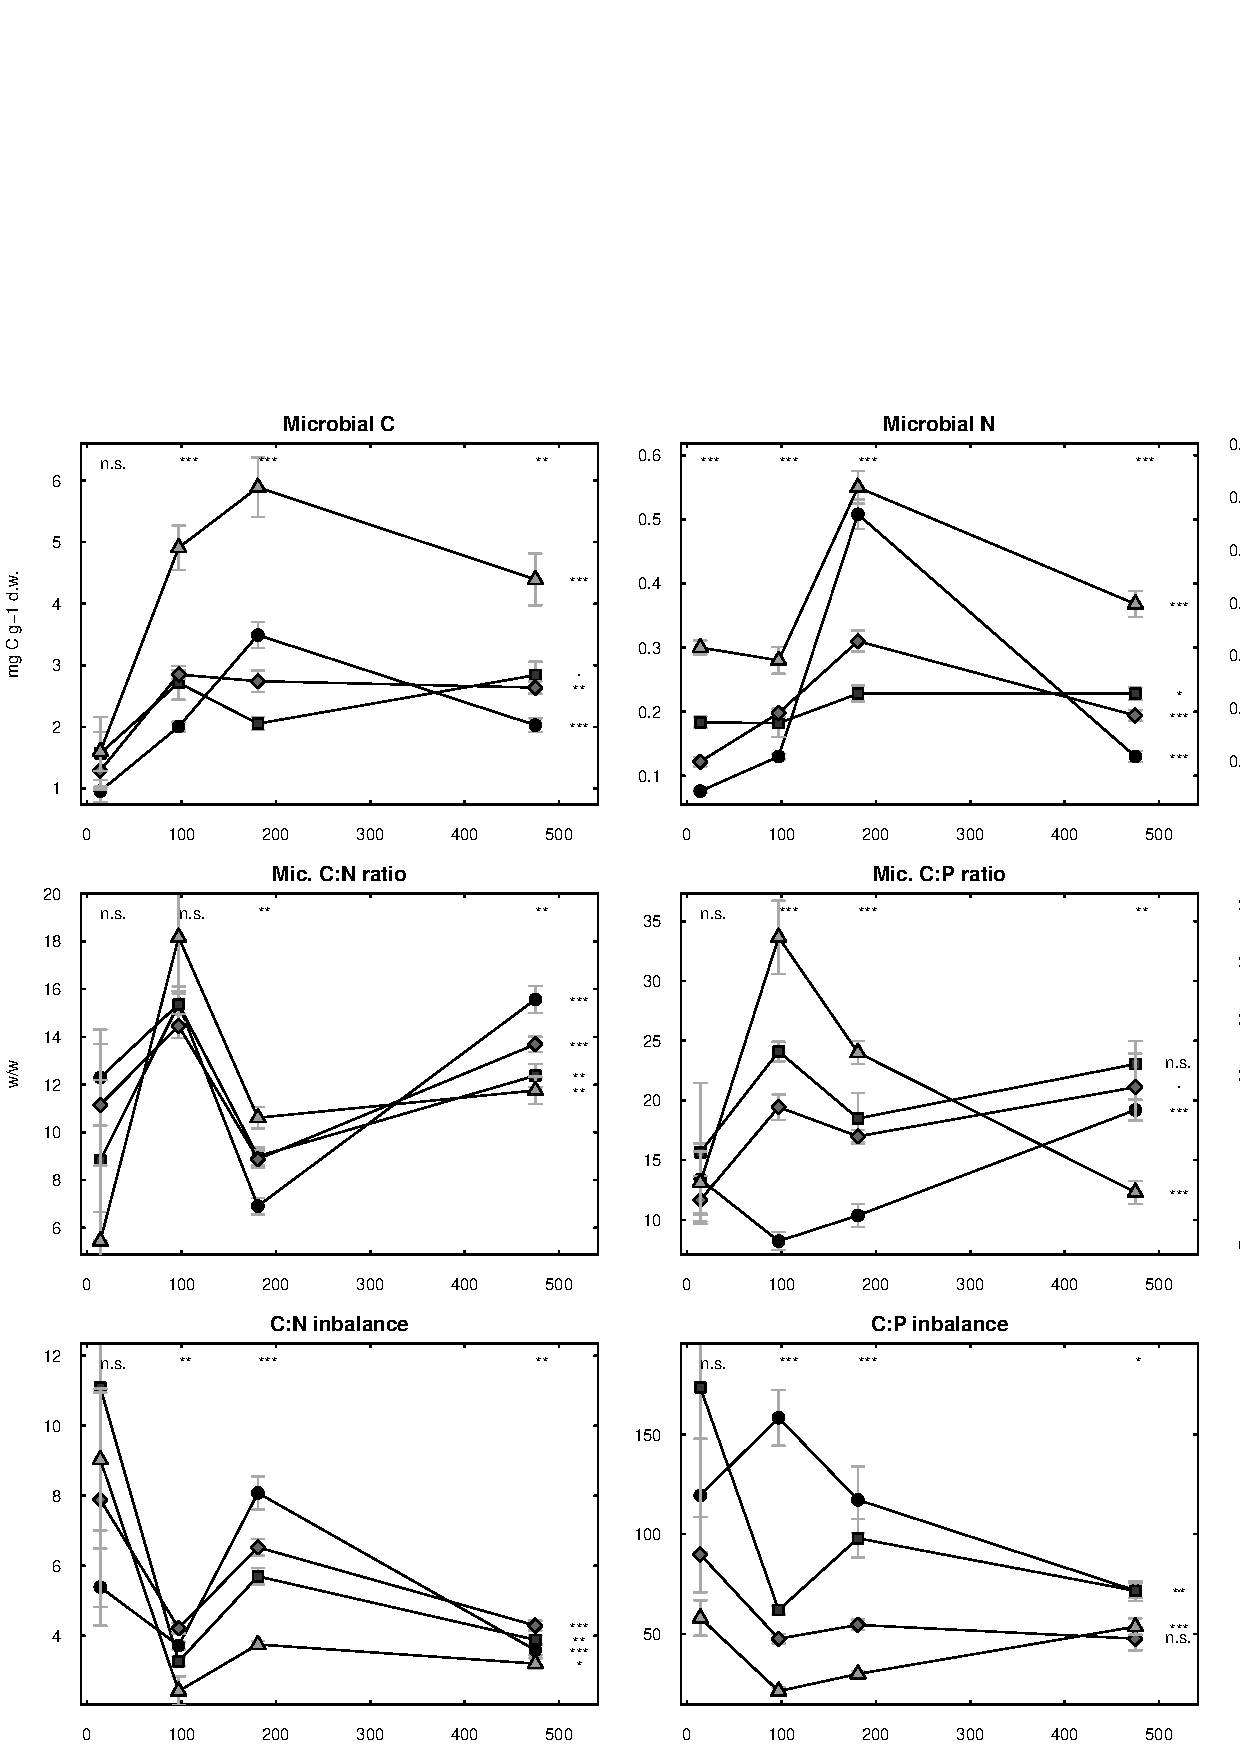
\includegraphics{sbb-mb}
\end{center}
\caption{Microbial biomassm, microbial stoichiometry and resource:consumer stoichiometric imbalance. Error bars indicate standard errors (n=5).}
\label{fig:mb}
\end{figure*}






\newpage
\begin{figure*}[h!]
\vspace*{2mm}
\begin{center}
\setkeys{Gin}{width=\textwidth}
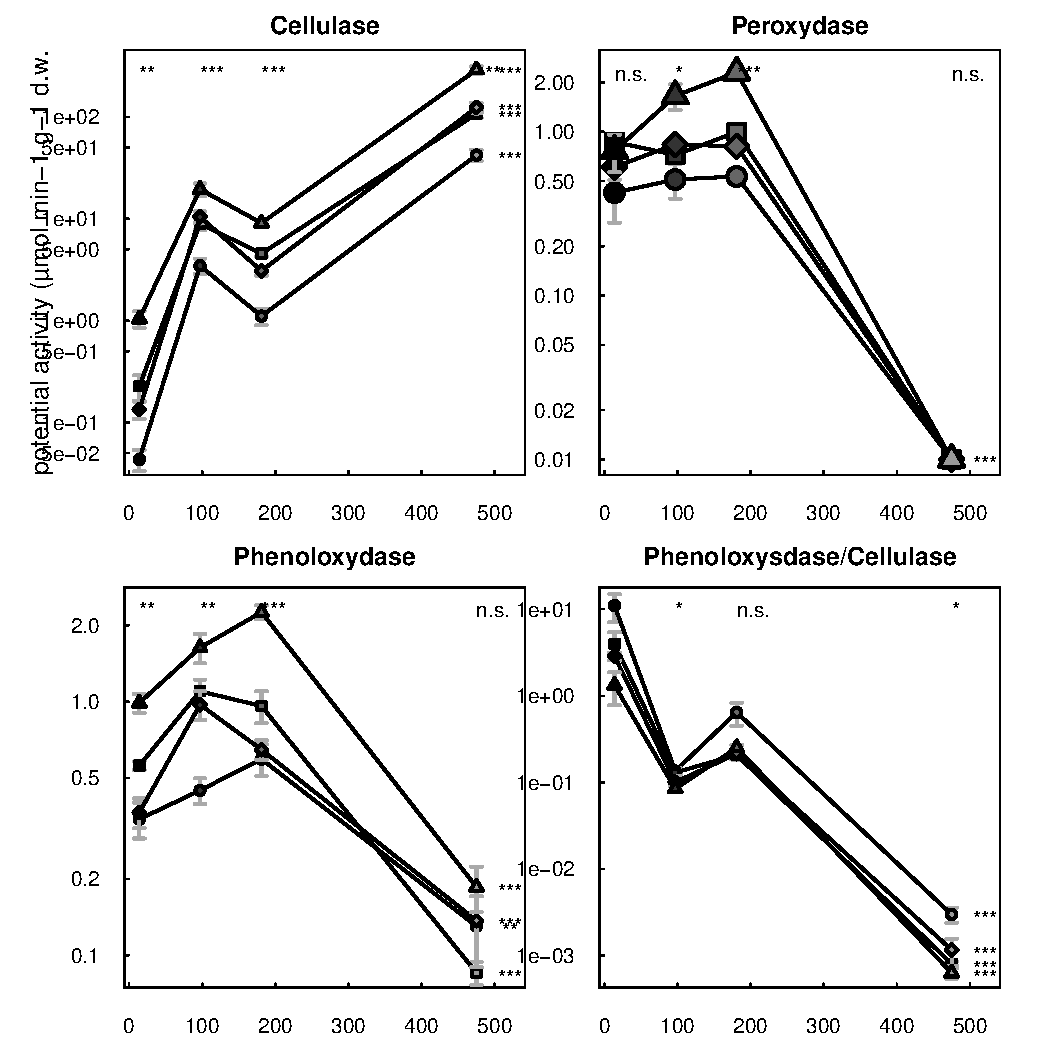
\includegraphics{sbb-enz}
\end{center}
\caption{Potential eco-enzyme activities}
\label{fig:enz}
\end{figure*}


%\newpage
%\begin{figure*}[h!]
%\vspace*{2mm}
%\begin{center}
%\setkeys{Gin}{width=\textwidth}
%<<pca2, fig=T, echo=F, results=hide>>=
%ord.plot(rda((rsim-initials.rsim)/initials.rsim, scale=T), days, type,scale=T, pt.bg=colscale, pch=pch, spe.labels=peakcodes, spe.mult=2.5, sep1.unit="days")
%@
%\end{center}
%\caption{Principal component analysis of the relative peak areas of 128 pyrolysis products, corrected by their abundance before incubation. Symbols indicate samples measured (means per litter type and time point), error bars indicate +/- 1 SE (n=4-5). Letters indicate pyrolysis products (L - lignin,  P - other phenolic compounds, C - carbohydrates, N - nitrogen containing compounds, open circles: nonspecific and unidentified peaks). Factor loadings of pyrolysis products were multiplied by 2.5 for better readability.}
%\label{fig:pca2}
%\end{figure*}

%\newpage
%\begin{figure*}[h!]
%\vspace*{2mm}
%\begin{center}
%\setkeys{Gin}{width=\textwidth}
%<<chemdif, fig=T, results=hide, echo=false>>=
%  par(mfrow=c(2,3))
%#barp(orig_cTIC$L, days==97, days==0)
%#barp(orig_cTIC$Ph, days==97, days==0)
%#barp(orig_cTIC$C, days==97, days==0)
%
%par(mar=c(0.6, 5, 2, 0))
%barp(orig_cTIC$L, days==181, days==0, ylim=c(-4,6), ylab="% TIC difference\n0-181 days", main="Lignin")
%#barp(orig_cTIC$Ph, days==181, days==97)
%axis(4, labels=F)
%
%par(mar=c(0.6, 0, 2, 5))
%#barp(orig_cTIC$Ph, days==181, days==97)
%barp(orig_cTIC$C, days==181, days==0, ylim=c(-4,6), yaxt="n", main="Carbohydrates")
%axis(4)
%axis(2, labels=F)
%#mtext("Carbohydrates degraded (% of initial pool)\n days 0 - 181", side=4, padj=2)
%#barpr(closs.corr.orig_cTIC$L, closs.corr.orig_cTIC$C, days==181, days==0, ylim=c(-1,3))
%
%par(mar=c(0.6, 0, 2, 5))
%barp(orig_cTIC$L/(orig_cTIC$L+orig_cTIC$C), days==181, days==0, ylim=c(-0.04,0.06), %main="LCI", yaxt="n")
%axis(4)
%axis(2, labels=F)
%mtext("LCI difference\n0-181 days", side=4, padj=3, las=0)
%
%par(mar=c(2, 5, 0.6,0))
%
%barp(orig_cTIC$L, days==475, days==181, ylim=c(-4,6), names.arg=typlev, ylab="% TIC difference\n181-475 days")
%#barp(orig_cTIC$Ph, days==475, days==181)
%axis(4, labels=F)litter quality
%
%par(mar=c(2, 0, 0.6,5))
%barp(orig_cTIC$C, days==475, days==181, yaxt="n", names.arg=typlev, ylim=c(-4,6))
%axis(4)
%axis(2, labels=F)
%
%par(mar=c(2, 0, 0.6,5))
%barp(orig_cTIC$L/(orig_cTIC$L+orig_cTIC$C), days==475, days==181, ylim=c(-0.04,0.06), names.arg=typlev, yaxt="n")
%axis(4)
%axis(2, labels=F)
%mtext("LCI difference\n181-475 days", side=4, padj=3, las=0)
%
%@
%\end{center}
%\caption{Accumulation and depletion of lignin and carbohydrates}
%\label{fig:chemdif}
%\end{figure*}

\newpage
\begin{figure*}[h!]
\vspace*{2mm}
\begin{center}
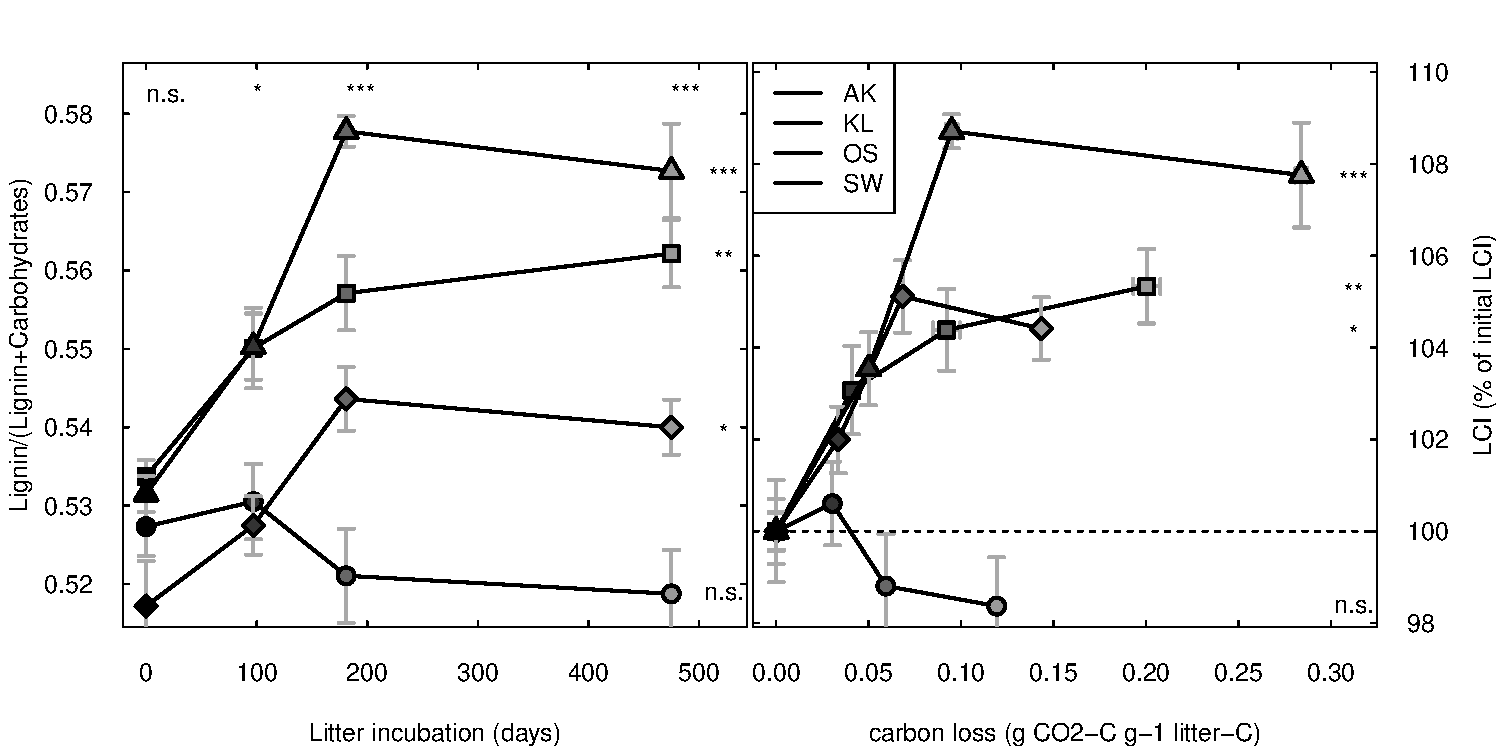
\includegraphics{sbb-lci}
\end{center}
\caption{Develoment of the LCI (lignin/(lignin+carbohydrates)). Errorbars indicate standard errors (n=4-5). The dashed line indicates a constant ratio between lignin and carbohydrates (i.e. no preferential decomposition of carbohydrates. )}
\label{fig:lci}
\end{figure*}

\newpage
\begin{figure*}[h!]
\vspace*{2mm}
\begin{center}
\setkeys{Gin}{width=\textwidth}
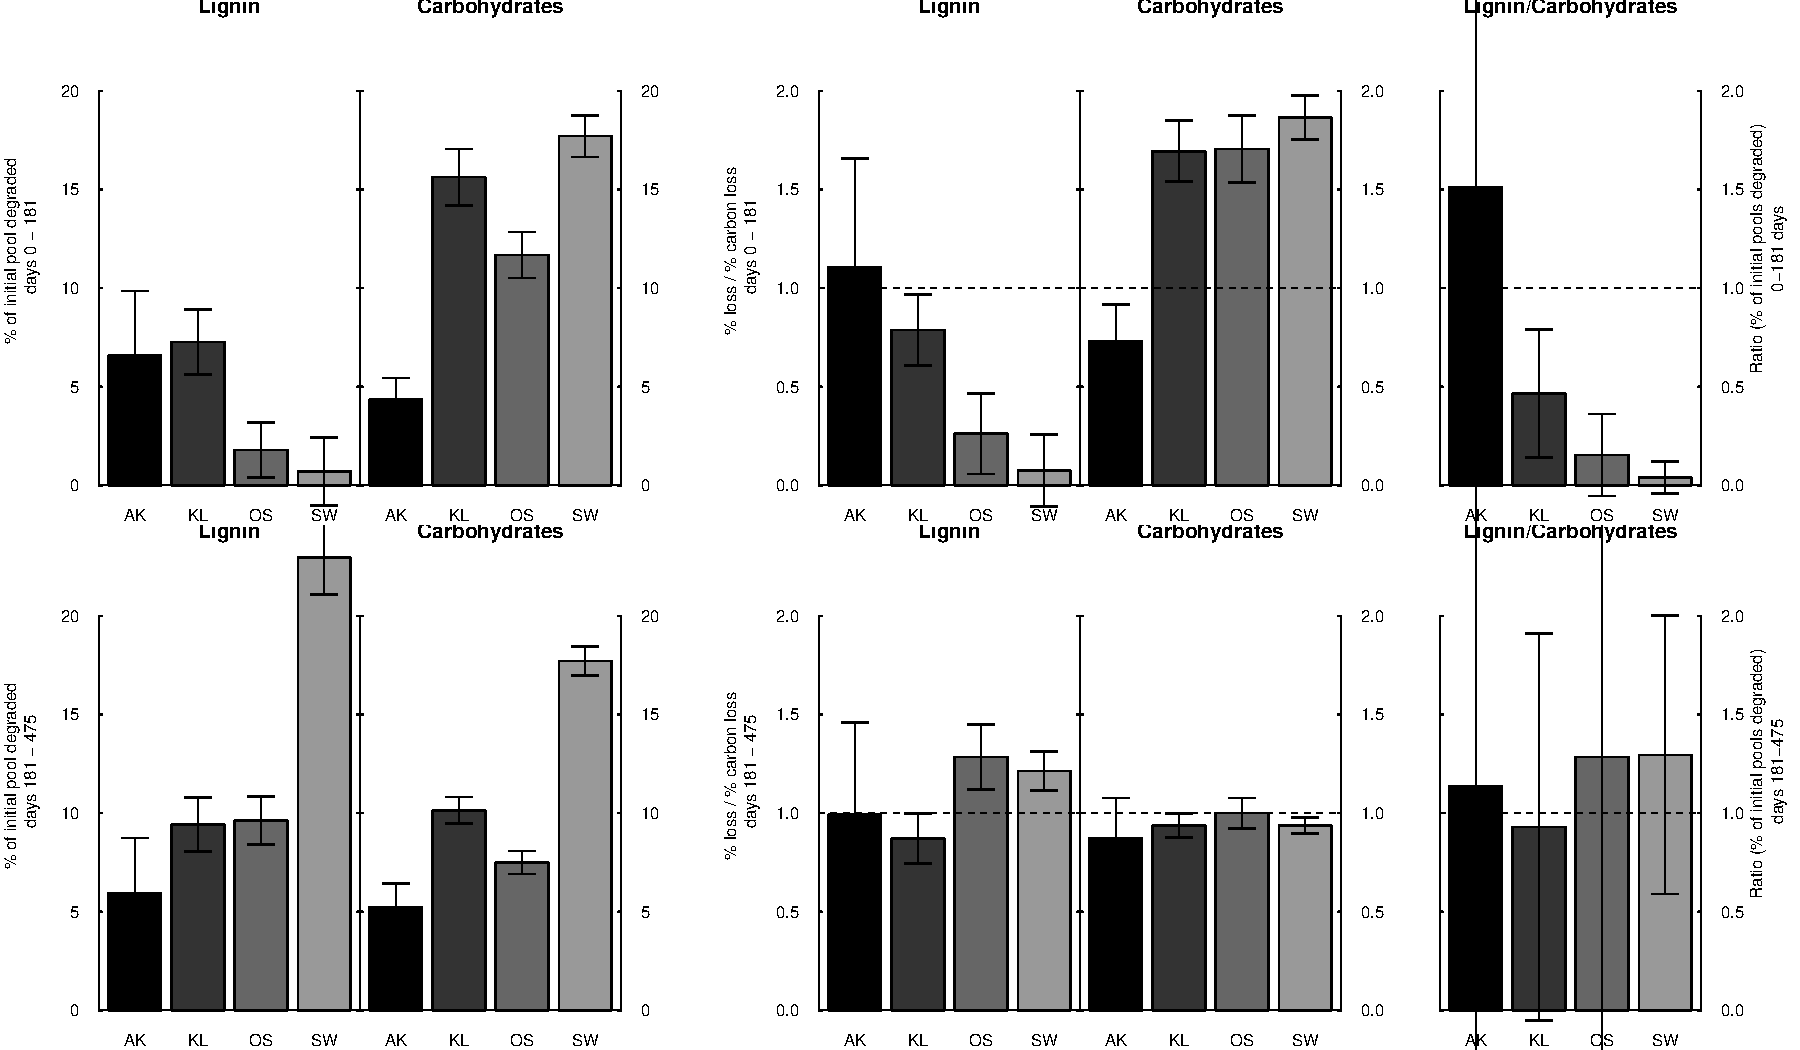
\includegraphics{sbb-degrdiff}
\end{center}
\caption{Carbon loss corrected amounts of lignin and carbohydrates degraded. Carbon loss was calculated based on accumulated respiration. Error bars indicate standard errors (n=4-5). The dashed line marks no discrination between lignin, carbohydrates and bulk carbon loss.}
\label{fig:degr}
\end{figure*}

\newpage
\begin{figure*}[h!]
\vspace*{2mm}
\begin{center}
\setkeys{Gin}{width=\textwidth}
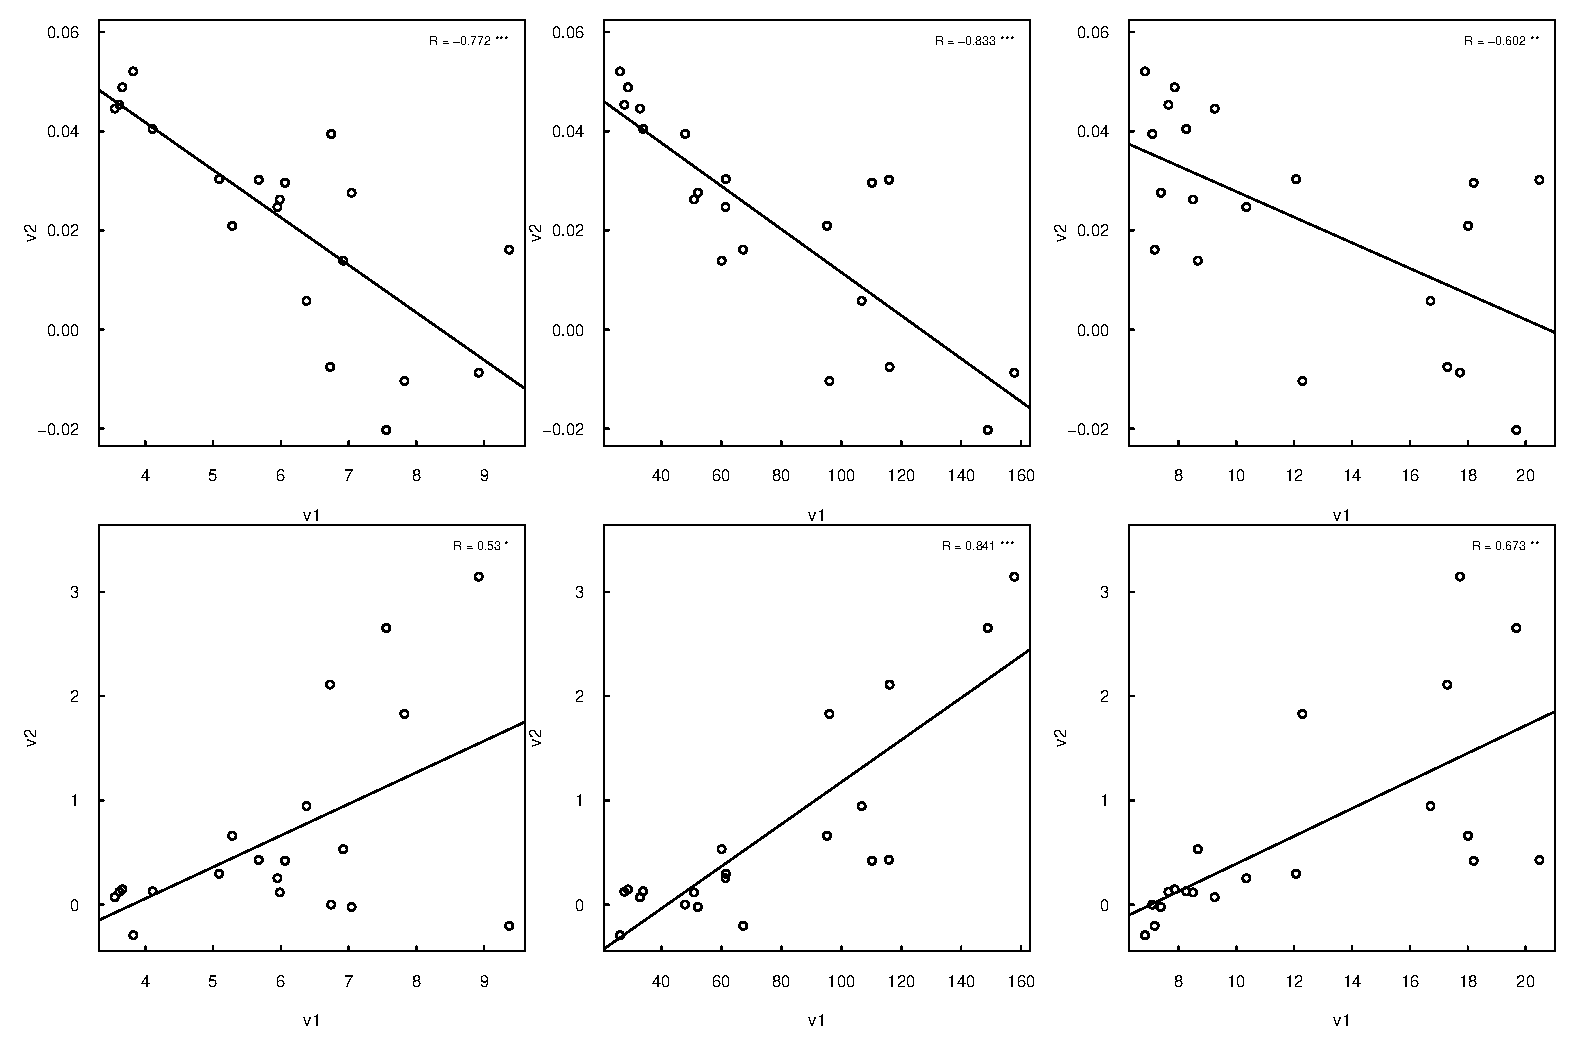
\includegraphics{sbb-graphcorr}
\end{center}
\caption{Correlations between Lignin accumulation during the first 6 month of litter incubation and stoichiometric resource:consumer imbalances}
\label{fig:cor1}
\end{figure*}

\newpage
\begin{figure*}[h!]
\vspace*{2mm}
\begin{center}
\setkeys{Gin}{width=\textwidth}
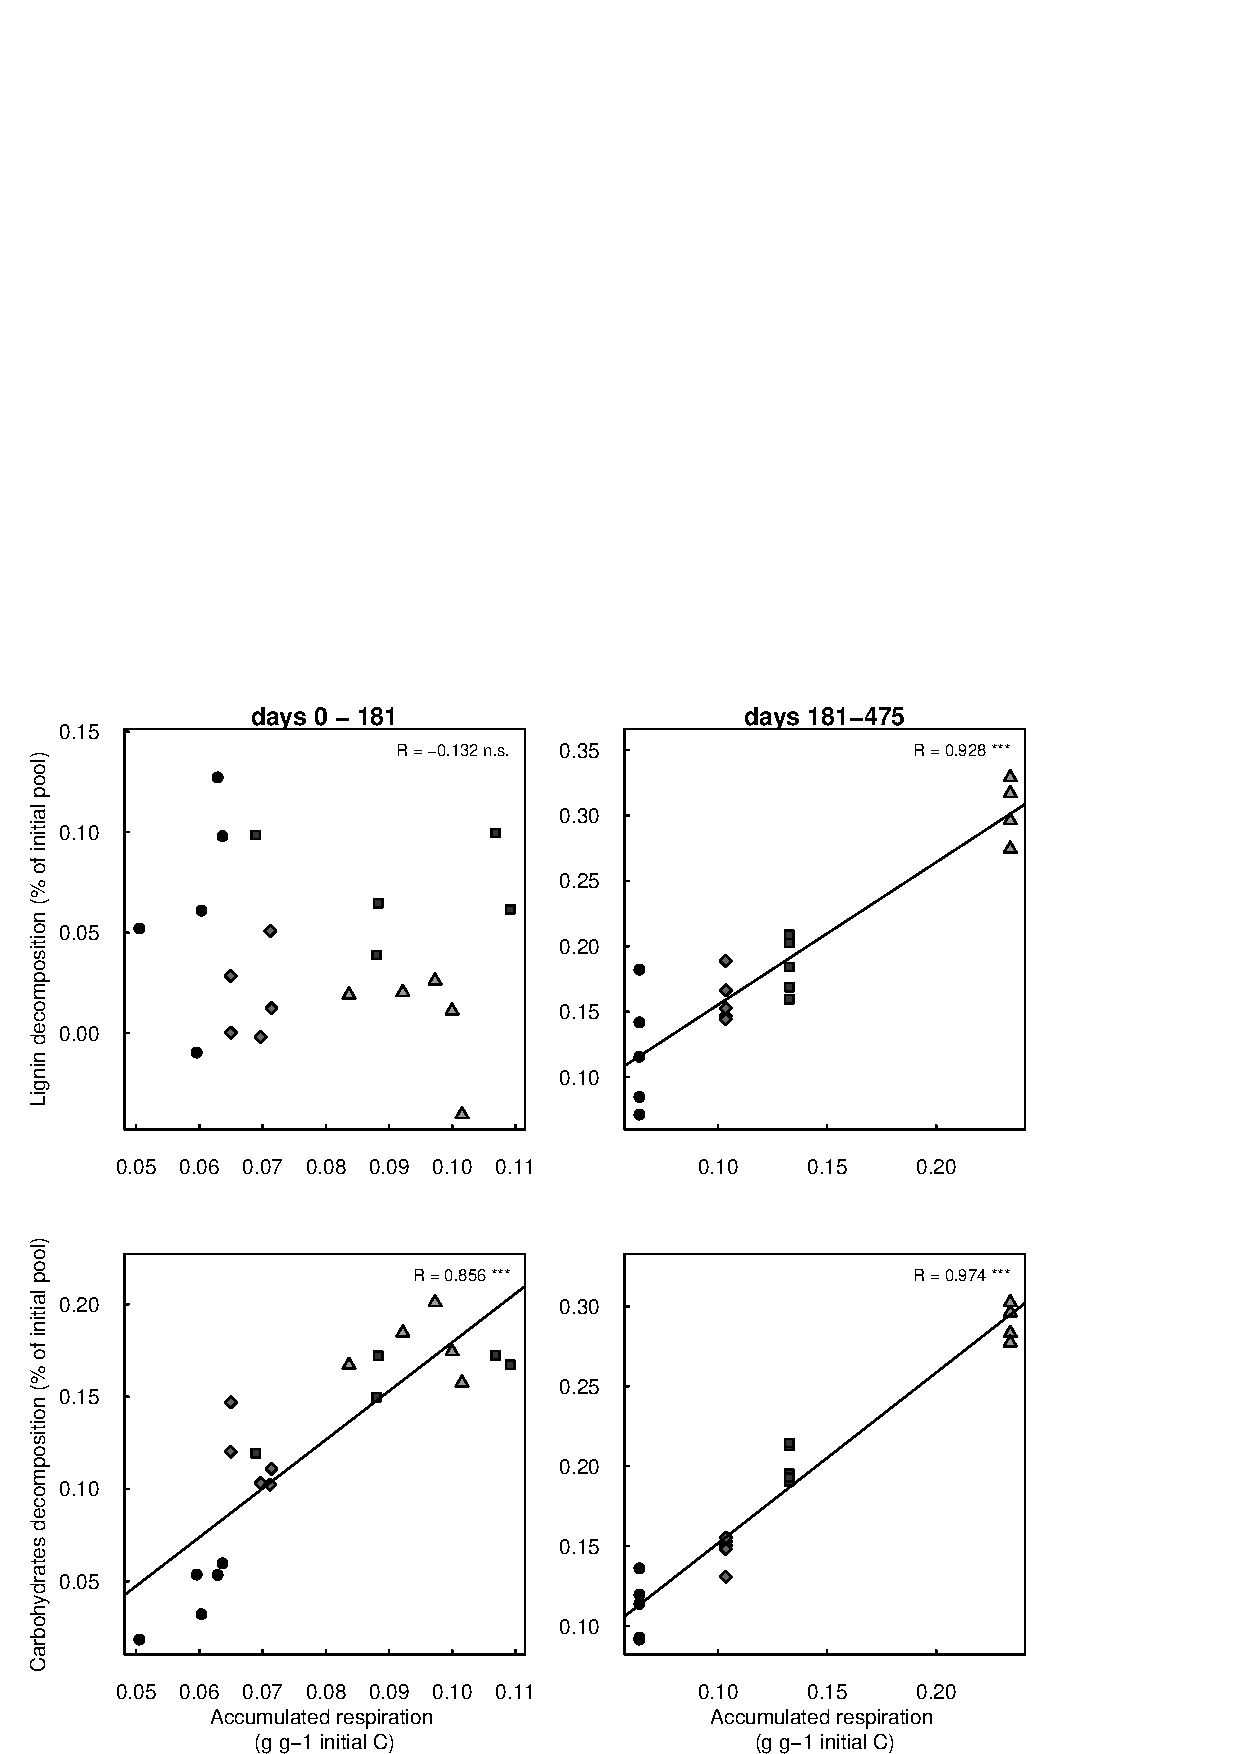
\includegraphics{sbb-respcorr}
\end{center}
\caption{caption}
\label{fig:repcor}
\end{figure*}

\newpage
\begin{figure*}[h!]
\vspace*{2mm}
\begin{center}
\setkeys{Gin}{width=\textwidth}
\includegraphics{sbb-enzcorr}
\end{center}
\caption{caption}
\label{fig:enzcor}
\end{figure*}


\newpage
\begin{figure*}[h!]
\vspace*{2mm}
\begin{center}
\setkeys{Gin}{width=\textwidth}
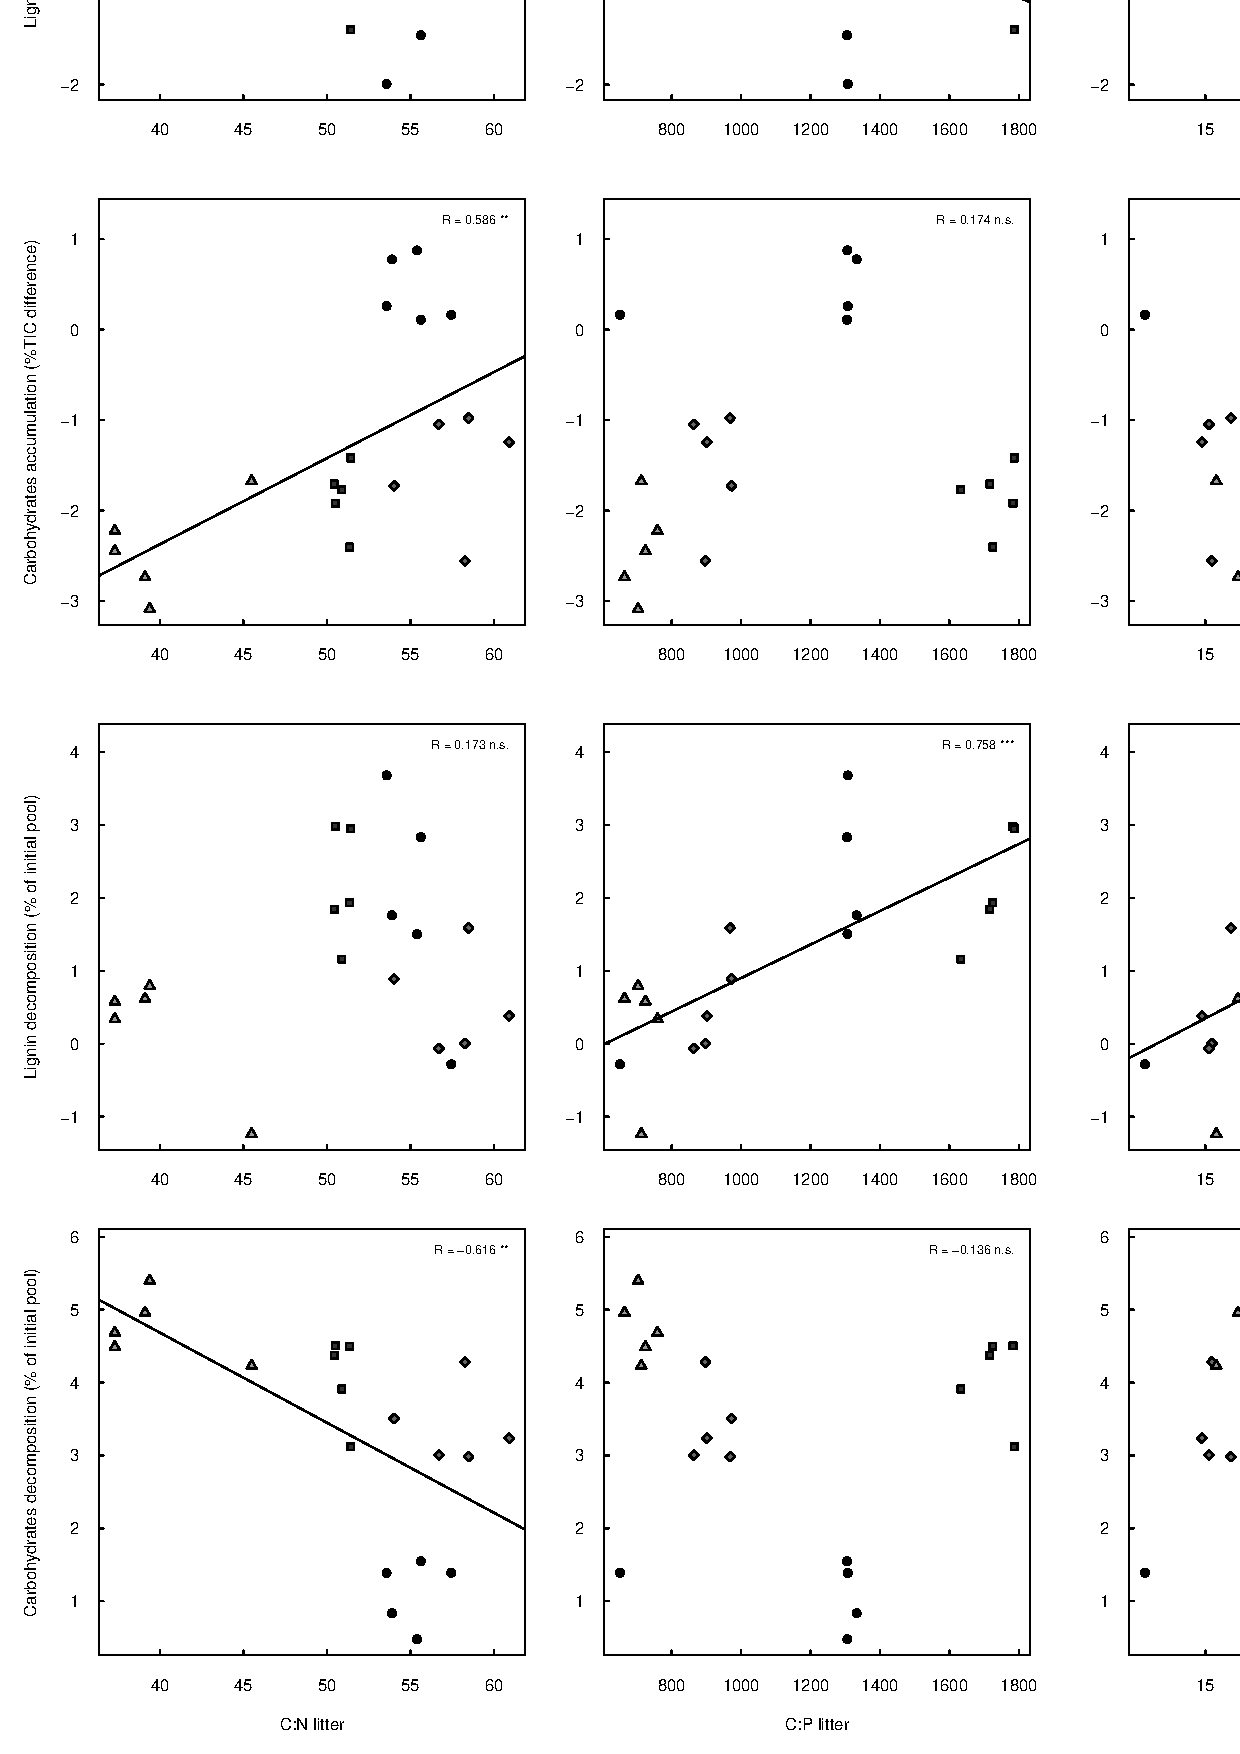
\includegraphics{sbb-graphcorr2}
\end{center}
\caption{Correlations between Lignin and Carbohydrates accumulation and decomposition during the first 6 month of litter incubation and litter C:N:P ratios}
\label{fig:cor2}
\end{figure*}

\newpage
\begin{figure*}[h!]
\vspace*{2mm}
\begin{center}
\setkeys{Gin}{width=\textwidth}
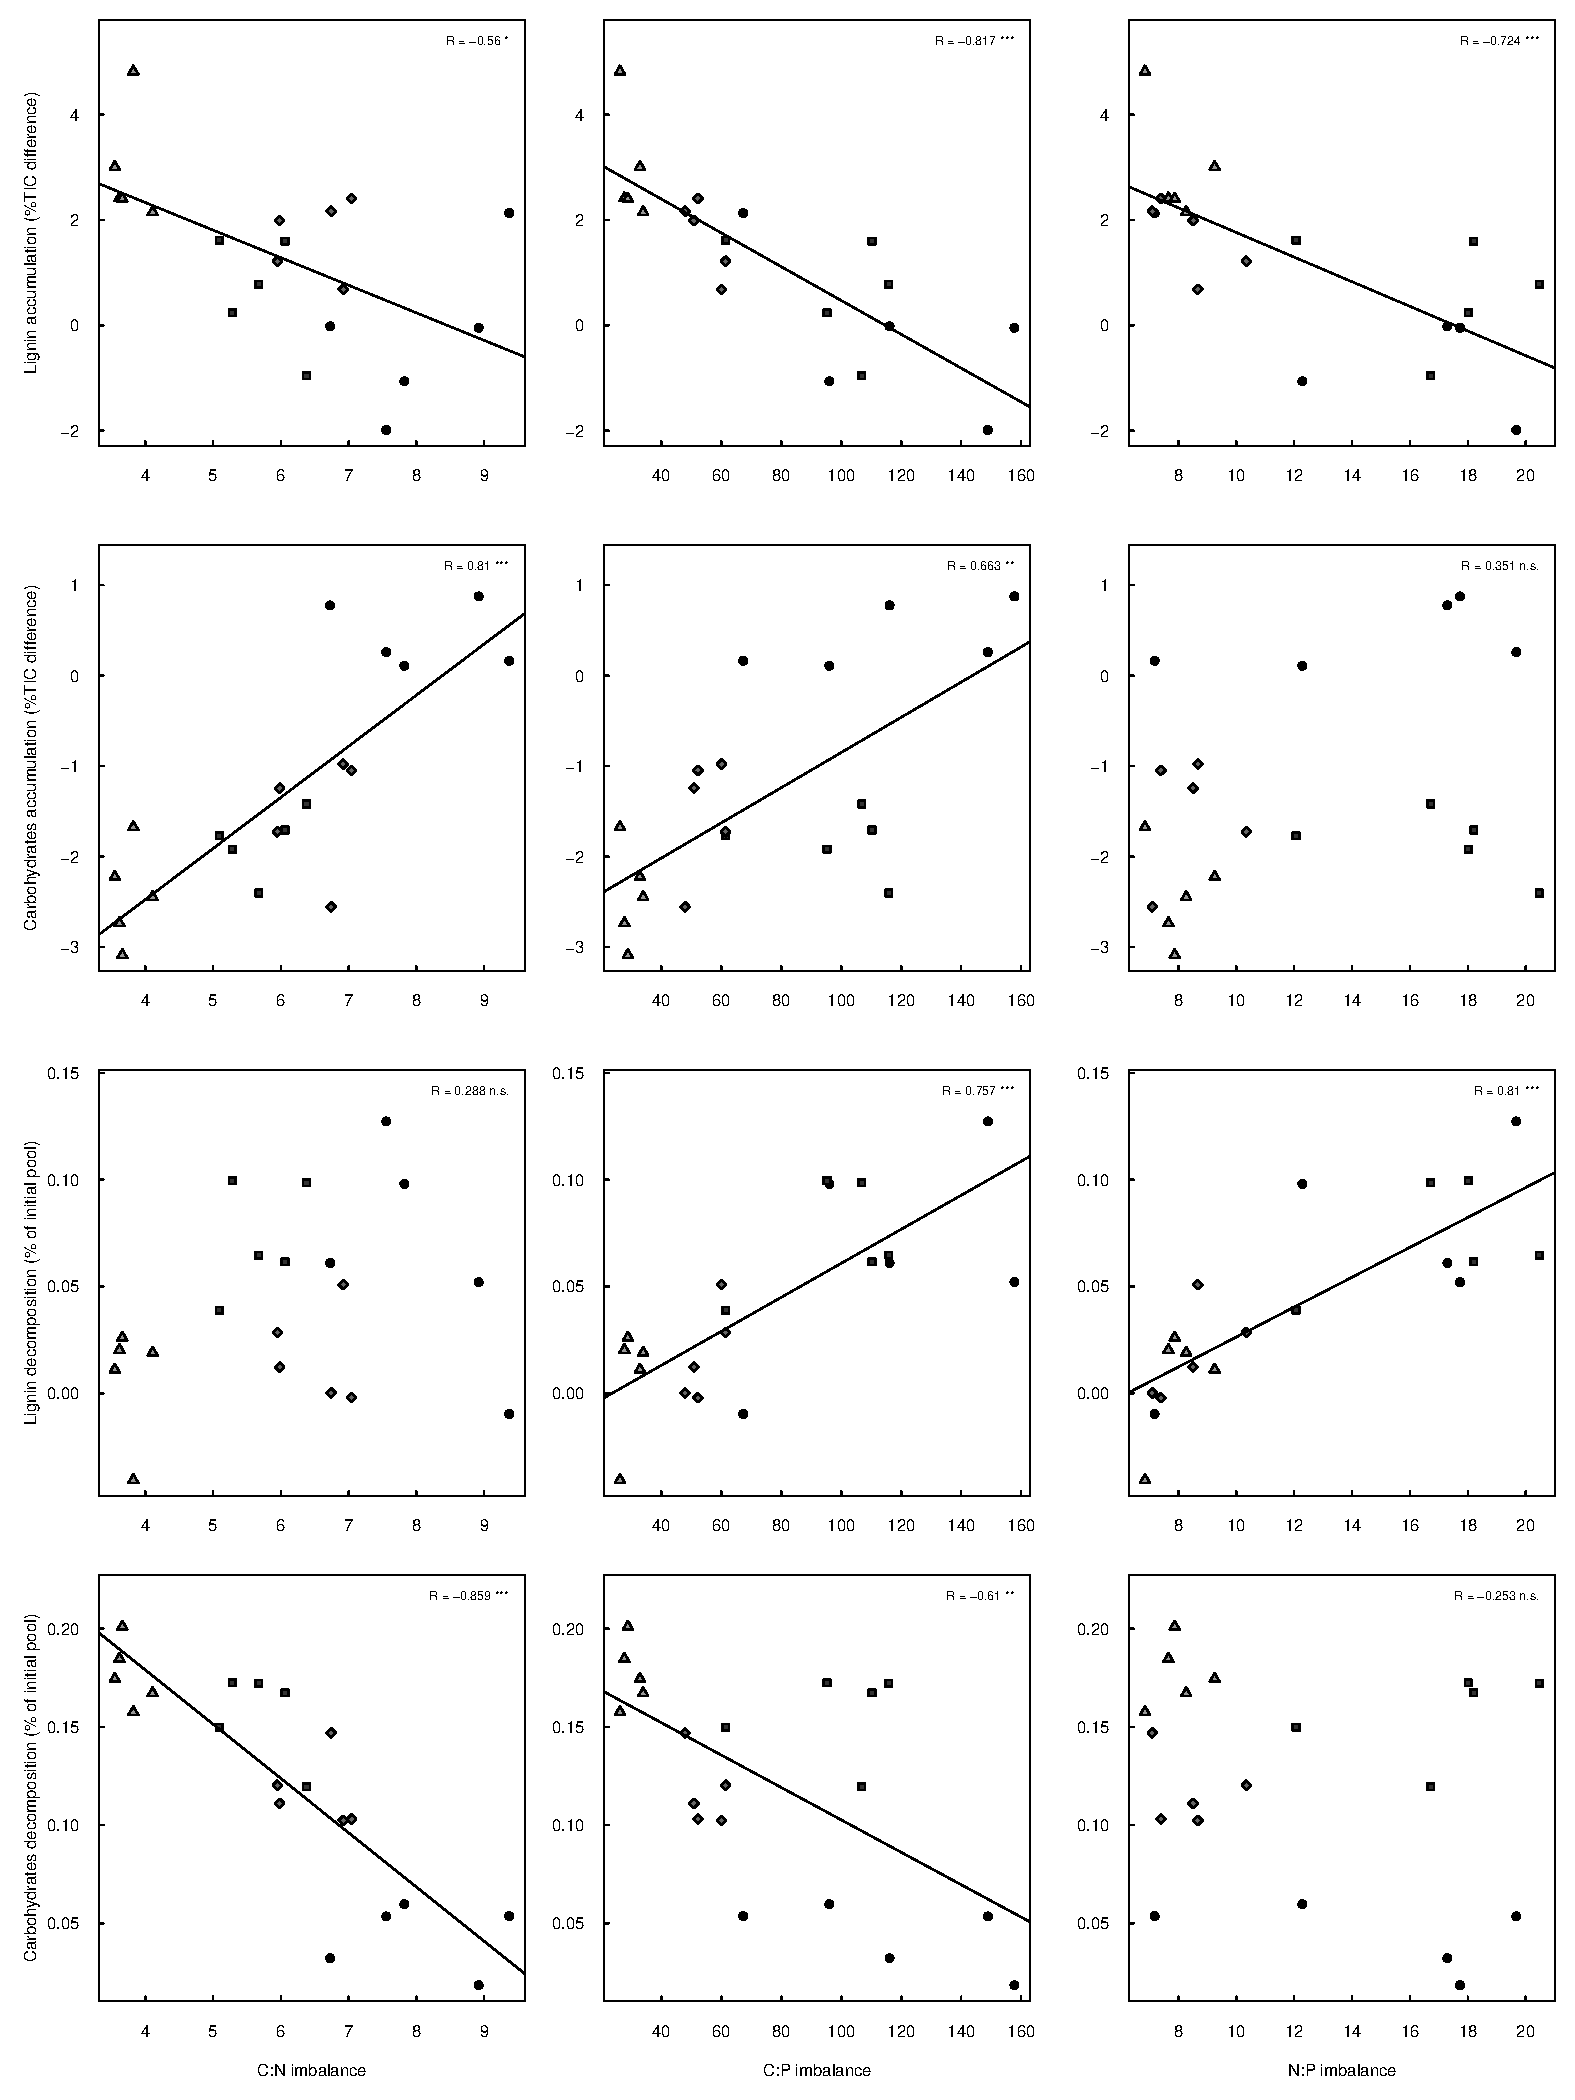
\includegraphics{sbb-graphcorr3}
\end{center}
\caption{Correlations between Lignin and Carbohydrates accumulation and decomposition during the first 6 month of litter incubation and stoichiometric resource:consumer imbalances}
\label{fig:cor3}
\end{figure*}


\newpage
% latex table generated in R 2.12.1 by xtable 1.6-0 package
% Thu Oct 20 11:29:54 2011
\begin{table}[h!]
\begin{center}
\caption{Litter stoichiometry and mineral elemental contents measured after 14 days incubation. Standard errors are stated in brackets (n=5). C extr stands for extractable carbon.}
\label{initstoech}
{\tiny
\begin{tabular}{cccccccccc}
  \hline
 & AK & (SE) & KL & (SE) & OS & (SE) & SW & (SE) & p value \\ 
  \hline
C (\% d.w.) & 50.86 & (0.39) & 49.41 & (0.53) & 48.15 & (0.39) & 48.90 & (0.34) & 0.002 \\ 
  C extr (mg g-1) & 0.46 & (0.03) & 0.14 & (0.01) & 0.21 & (0.01) & 0.64 & (0.03) & 0.002 \\ 
  N (\% d.w.) & 0.878 &  (0.012) & 0.938 &  (0.012) & 0.806 &  (0.013) & 1.172 &  (0.016) & $<$0.001 \\ 
  P (\% d.w.) & 0.040 & (0.000) & 0.030 & (0.000) & 0.052 & (0.002) & 0.070 & (0.000) & $<$0.001 \\ 
  C:N (w/w) & 57.86 &  (0.57) & 52.60 &  (0.49) & 59.97 &  (0.72) & 41.78 &  (0.76) & $<$0.001 \\ 
  C:P (w/w) & 1282 & (21) & 1548 & (25) & 905 & (15) & 699 & (9) & $<$0.001 \\ 
  N:P (w/w) & 22.17 & (0.47) & 29.45 & (0.60) & 15.10 & (0.29) & 16.75 & (0.39) & $<$0.001 \\ 
  K (mg g-1) & 0.26 & (0.00) & 0.54 & (0.00) & 0.21 & (0.00) & 0.55 & (0.00) & $<$0.001 \\ 
  Ca (mg g-1) & 1.33 & (0.01) & 1.26 & (0.01) & 1.63 & (0.01) & 1.23 & (0.01) & $<$0.001 \\ 
  Mg (mg g-1) & 0.27 &  (0.00) & 0.14 &  (0.00) & 0.20 &  (0.00) & 0.15 &  (0.00) & $<$0.001 \\ 
  Fe (ppm) & 210 & (2) & 208 & (4) & 453 & (12) & 192 & (4) & $<$0.001 \\ 
  Mn (ppm) & 172 &  (2) & 1430 &  (10) & 776 &  (9) & 2137 &  (51) & $<$0.001 \\ 
  Zn (ppm) & 30.8 & (0.4) & 33.0 & (0.3) & 36.0 & (1.0) & 42.4 & (0.7) & $<$0.001 \\ 
   \hline
\end{tabular}
}
\end{center}
\end{table}
\newpage
% latex table generated in R 2.12.1 by xtable 1.6-0 package
% Thu Oct 20 11:29:54 2011
\begin{table}[h!]
\begin{center}
\caption{Correlation (R) between Lignin and Carbohydrate degration with litter chemistry, microbial community and decomposition processes. Significant (p<0.05) correlations are printed bold. Data taken from \cite{Mooshammer2011, Leitner2011}. Differences in litter chemistry were calculaten between 0 and 181 days, process rates were measured after 181 days.}
\label{corrtable}
{\tiny
\begin{tabular}{ccccccccccc}
  \hline
 & L acc & Ch acc & LCI diff & L dec & C dec & L resp & C resp & L/C dec & Per/Cell & Phen/Cell \\ 
  \hline
Massloss & 0.291 & -0.15 & 0.245 & -0.339 & 0.0964 & -0.211 & 0.0965 & -0.0818 & 0.048 & 0.0534 \\ 
  Actual respiration & 0.333 & \textbf{ -0.723 } & \textbf{ 0.606 } & -0.0747 & \textbf{ 0.732 } & -0.19 & \textbf{ 0.507 } & -0.364 & -0.268 & -0.362 \\ 
  Accumulated Respiration & \textbf{ 0.494 } & \textbf{ -0.704 } & \textbf{ 0.688 } & -0.123 & \textbf{ 0.82 } & -0.327 & \textbf{ 0.483 } & \textbf{ -0.522 } & \textbf{ -0.506 } & \textbf{ -0.534 } \\ 
  Cellulase activity & \textbf{ 0.657 } & \textbf{ -0.76 } & \textbf{ 0.803 } & -0.424 & \textbf{ 0.789 } & \textbf{ -0.493 } & \textbf{ 0.611 } & \textbf{ -0.588 } & -0.436 & \textbf{ -0.539 } \\ 
  Protease activity & 0.186 & -0.296 & 0.264 & -0.123 & 0.295 & -0.148 & 0.314 & -0.272 & -0.26 & -0.18 \\ 
  Chitinase activity & 0.409 & \textbf{ -0.749 } & \textbf{ 0.663 } & -0.157 & \textbf{ 0.766 } & -0.301 & \textbf{ 0.604 } & \textbf{ -0.555 } & \textbf{ -0.49 } & \textbf{ -0.607 } \\ 
  Phosphatase activity & \textbf{ 0.549 } & \textbf{ -0.813 } & \textbf{ 0.776 } & -0.292 & \textbf{ 0.832 } & -0.4 & \textbf{ 0.638 } & \textbf{ -0.554 } & -0.418 & \textbf{ -0.522 } \\ 
  Phenoloxidase activity & \textbf{ 0.632 } & \textbf{ -0.669 } & \textbf{ 0.737 } & -0.412 & \textbf{ 0.708 } & \textbf{ -0.448 } & \textbf{ 0.503 } & \textbf{ -0.484 } & -0.305 & -0.356 \\ 
  Peroxidase activity & \textbf{ 0.599 } & \textbf{ -0.588 } & \textbf{ 0.677 } & -0.41 & \textbf{ 0.618 } & -0.439 & 0.412 & -0.435 & -0.173 & -0.302 \\ 
  N mineralization & \textbf{ 0.466 } & \textbf{ -0.664 } & \textbf{ 0.65 } & -0.159 & \textbf{ 0.703 } & -0.295 & 0.45 & -0.384 & -0.282 & -0.367 \\ 
  Nitrification & \textbf{ 0.587 } & \textbf{ -0.707 } & \textbf{ 0.732 } & -0.377 & \textbf{ 0.721 } & -0.431 & \textbf{ 0.565 } & \textbf{ -0.497 } & -0.369 & -0.45 \\ 
  P mineralization & \textbf{ 0.665 } & \textbf{ -0.55 } & \textbf{ 0.684 } & \textbf{ -0.544 } & \textbf{ 0.59 } & \textbf{ -0.58 } & 0.387 & \textbf{ -0.479 } & -0.212 & -0.255 \\ 
  C litter & \textbf{ -0.545 } & \textbf{ 0.506 } & \textbf{ -0.578 } & \textbf{ 0.589 } & \textbf{ -0.45 } & \textbf{ 0.631 } & \textbf{ -0.704 } & \textbf{ 0.702 } & \textbf{ 0.525 } & \textbf{ 0.581 } \\ 
  extractable C & \textbf{ 0.609 } & \textbf{ -0.766 } & \textbf{ 0.782 } & -0.364 & \textbf{ 0.793 } & -0.443 & \textbf{ 0.593 } & \textbf{ -0.538 } & -0.392 & \textbf{ -0.484 } \\ 
  N litter & 0.354 & \textbf{ -0.517 } & \textbf{ 0.503 } & -0.14 & \textbf{ 0.546 } & -0.189 & 0.286 & -0.201 & -0.119 & -0.159 \\ 
  P litter & \textbf{ 0.682 } & -0.222 & \textbf{ 0.517 } & \textbf{ -0.75 } & 0.204 & \textbf{ -0.686 } & 0.211 & \textbf{ -0.496 } & -0.0728 & -0.16 \\ 
  C:N litter & -0.405 & \textbf{ 0.586 } & \textbf{ -0.57 } & 0.173 & \textbf{ -0.616 } & 0.234 & -0.36 & 0.271 & 0.195 & 0.242 \\ 
  C:P litter & \textbf{ -0.636 } & 0.174 & \textbf{ -0.453 } & \textbf{ 0.758 } & -0.136 & \textbf{ 0.655 } & -0.234 & 0.425 & 0.049 & 0.0805 \\ 
  N:P litter & \textbf{ -0.512 } & -0.0287 & -0.264 & \textbf{ 0.718 } & 0.079 & \textbf{ 0.583 } & -0.107 & 0.324 & -0.0316 & -0.0192 \\ 
  C:N mic & \textbf{ 0.666 } & \textbf{ -0.758 } & \textbf{ 0.799 } & -0.423 & \textbf{ 0.807 } & \textbf{ -0.511 } & \textbf{ 0.657 } & \textbf{ -0.609 } & \textbf{ -0.584 } & \textbf{ -0.596 } \\ 
  C:P mic & \textbf{ 0.692 } & \textbf{ -0.787 } & \textbf{ 0.834 } & \textbf{ -0.468 } & \textbf{ 0.818 } & \textbf{ -0.557 } & \textbf{ 0.694 } & \textbf{ -0.671 } & \textbf{ -0.564 } & \textbf{ -0.648 } \\ 
  N:P mic & \textbf{ 0.582 } & \textbf{ -0.729 } & \textbf{ 0.74 } & -0.406 & \textbf{ 0.733 } & \textbf{ -0.502 } & \textbf{ 0.685 } & \textbf{ -0.669 } & \textbf{ -0.545 } & \textbf{ -0.671 } \\ 
  C:N imbalance & \textbf{ -0.56 } & \textbf{ 0.81 } & \textbf{ -0.772 } & 0.28 & \textbf{ -0.851 } & 0.386 & \textbf{ -0.662 } & \textbf{ 0.53 } & \textbf{ 0.564 } & \textbf{ 0.56 } \\ 
  C:P imbalance & \textbf{ -0.817 } & \textbf{ 0.663 } & \textbf{ -0.833 } & \textbf{ 0.748 } & \textbf{ -0.653 } & \textbf{ 0.794 } & \textbf{ -0.691 } & \textbf{ 0.841 } & \textbf{ 0.575 } & \textbf{ 0.67 } \\ 
  N:P imbalance & \textbf{ -0.724 } & 0.351 & \textbf{ -0.602 } & \textbf{ 0.807 } & -0.313 & \textbf{ 0.763 } & \textbf{ -0.455 } & \textbf{ 0.673 } & 0.301 & 0.41 \\ 
   \hline
\end{tabular}
}
\end{center}
\end{table}
\newpage
% latex table generated in R 2.12.1 by xtable 1.6-0 package
% Thu Oct 20 11:29:55 2011
\begin{table}[h!]
\begin{center}
\caption{Correlation (R) between Lignin and Carbohydrate degration with litter chemistry, microbial community and decomposition processes. Significant (p<0.05) correlations are printed bold. Data taken from \cite{Mooshammer2011, Leitner2011}. Differences in litter chemistry were calculaten between 181 and 475 days, process rates were measured after 475 days.}
\label{corrtable2}
{\tiny
\begin{tabular}{ccccccccccc}
  \hline
 & L acc & Ch acc & LCI diff & L dec & C dec & L resp & C resp & L/C dec & Per/Cell & Phen/Cell \\ 
  \hline
Massloss & -0.0455 & -0.264 & 0.0665 & \textbf{ 0.608 } & \textbf{ 0.685 } & \textbf{ 0.49 } & 0.436 & -0.144 & -0.444 & 0.403 \\ 
  Actual respiration & -0.374 & -0.22 & -0.213 & \textbf{ 0.882 } & \textbf{ 0.84 } & \textbf{ 0.84 } & \textbf{ 0.771 } & -0.293 & -0.403 & 0.29 \\ 
  Accumulated Respiration & -0.165 & -0.29 & -0.0113 & \textbf{ 0.91 } & \textbf{ 0.965 } & \textbf{ 0.752 } & \textbf{ 0.765 } & -0.409 & \textbf{ -0.608 } & \textbf{ 0.486 } \\ 
  Cellulase activity & -0.317 & -0.307 & -0.137 & \textbf{ 0.891 } & \textbf{ 0.887 } & \textbf{ 0.82 } & \textbf{ 0.885 } & -0.442 & \textbf{ -0.575 } & 0.414 \\ 
  Protease activity & -0.229 & -0.271 & -0.086 & \textbf{ 0.493 } & \textbf{ 0.495 } & \textbf{ 0.463 } & \textbf{ 0.664 } & \textbf{ -0.475 } & \textbf{ -0.456 } & 0.381 \\ 
  Phosphatase activity & 0.0425 & -0.0182 & 0.0685 & 0.368 & 0.405 & 0.285 & \textbf{ 0.489 } & -0.408 & -0.152 & 0.0167 \\ 
  Chitinase activity & -0.221 & -0.228 & -0.0874 & \textbf{ 0.717 } & \textbf{ 0.719 } & \textbf{ 0.606 } & \textbf{ 0.771 } & \textbf{ -0.543 } & \textbf{ -0.58 } & 0.395 \\ 
  Phenoloxidase activity & 0.34 & -0.436 & 0.435 & -0.218 & 0.00927 & -0.346 & -0.134 & -0.184 & \textbf{ -0.483 } & \textbf{ 0.692 } \\ 
  Peroxidase activity & -0.274 & 0.452 & -0.385 & 0.148 & -0.0609 & 0.269 & 0.0763 & 0.17 & \textbf{ 0.546 } & \textbf{ -0.708 } \\ 
  N mineralization & 0.175 & 0.195 & 0.0757 & 0.0241 & 0.0543 & -0.0988 & -0.189 & 0.0091 & 0.0624 & 0.0892 \\ 
  Nitrification & -0.289 & 0.23 & -0.321 & \textbf{ 0.631 } & \textbf{ 0.54 } & \textbf{ 0.559 } & 0.352 & 0.0392 & -0.105 & -0.0234 \\ 
  P mineralization & -0.164 & 0.0616 & -0.137 & \textbf{ 0.497 } & \textbf{ 0.458 } & \textbf{ 0.505 } & 0.367 & -0.0317 & 0.0433 & -0.0273 \\ 
  C litter & 0.33 & 0.231 & 0.176 & -0.392 & -0.346 & -0.413 & \textbf{ -0.713 } & \textbf{ 0.639 } & \textbf{ 0.501 } & -0.348 \\ 
  extractable C & -0.205 & -0.188 & -0.0882 & \textbf{ 0.88 } & \textbf{ 0.894 } & \textbf{ 0.727 } & \textbf{ 0.717 } & -0.366 & \textbf{ -0.538 } & 0.409 \\ 
  N litter & -0.17 & -0.166 & -0.0672 & \textbf{ 0.838 } & \textbf{ 0.861 } & \textbf{ 0.702 } & \textbf{ 0.567 } & -0.153 & -0.431 & 0.349 \\ 
  P litter & -0.4 & -0.369 & -0.181 & \textbf{ 0.782 } & \textbf{ 0.756 } & \textbf{ 0.806 } & \textbf{ 0.885 } & -0.399 & \textbf{ -0.464 } & 0.325 \\ 
  C:N litter & 0.124 & 0.196 & 0.018 & \textbf{ -0.827 } & \textbf{ -0.874 } & \textbf{ -0.664 } & \textbf{ -0.564 } & 0.194 & \textbf{ 0.49 } & -0.404 \\ 
  C:P litter & \textbf{ 0.508 } & 0.277 & 0.313 & \textbf{ -0.637 } & \textbf{ -0.538 } & \textbf{ -0.746 } & \textbf{ -0.793 } & 0.292 & 0.283 & -0.162 \\ 
  N:P litter & \textbf{ 0.477 } & 0.189 & 0.325 & -0.307 & -0.179 & \textbf{ -0.496 } & \textbf{ -0.56 } & 0.171 & 0.048 & 0.0338 \\ 
  C:N mic & 0.216 & 0.186 & 0.095 & \textbf{ -0.728 } & \textbf{ -0.741 } & \textbf{ -0.582 } & \textbf{ -0.661 } & \textbf{ 0.557 } & \textbf{ 0.57 } & \textbf{ -0.513 } \\ 
  C:P mic & 0.395 & 0.0762 & 0.312 & \textbf{ -0.565 } & \textbf{ -0.466 } & \textbf{ -0.584 } & -0.426 & -0.0723 & 0.233 & -0.223 \\ 
  N:P mic & 0.333 & 0.0142 & 0.288 & -0.298 & -0.189 & -0.389 & -0.199 & -0.287 & -0.00191 & -0.00931 \\ 
  C:N imbalance & -0.0522 & 0.084 & -0.0756 & -0.322 & -0.37 & -0.273 & -0.0657 & -0.317 & 0.0273 & 0.0196 \\ 
  C:P imbalance & 0.0913 & 0.335 & -0.0757 & -0.189 & -0.234 & -0.264 & \textbf{ -0.552 } & \textbf{ 0.493 } & 0.16 & -0.0317 \\ 
  N:P imbalance & 0.0576 & 0.293 & -0.0865 & -0.027 & -0.0722 & -0.0929 & \textbf{ -0.464 } & \textbf{ 0.615 } & 0.16 & -0.0803 \\ 
   \hline
\end{tabular}
}
\end{center}
\end{table}
\newpage
\begin{landscape}
% latex table generated in R 2.12.1 by xtable 1.6-0 package
% Thu Oct 20 11:29:55 2011
\begin{table}[h!]
\begin{center}
\caption{Correlations between C25/27/29 alkanes and alkenes, 14:0, 16:0 and 18:0 fatty acids and phytol. Differences between 0 and 181 days.}
\label{corrtable_notlig}
{\tiny
\begin{tabular}{ccccccccccccc}
  \hline
 & alkanacc & alkenacc & faacc & phytolacc & alkandeg & alkendeg & fadeg & phytoldeg & alkanresp & alkenresp & faresp & phytolresp \\ 
  \hline
Massloss & 0.17 & \textbf{ 0.49 } & -0.0933 & 0.226 & -0.18 & \textbf{ -0.45 } & 0.114 & -0.213 & -0.255 & -0.356 & 0.0694 & -0.114 \\ 
  Actual respiration & \textbf{ 0.752 } & 0.428 & \textbf{ 0.701 } & \textbf{ 0.792 } & \textbf{ -0.715 } & -0.202 & \textbf{ -0.673 } & \textbf{ -0.775 } & \textbf{ -0.491 } & 0.00695 & \textbf{ -0.699 } & \textbf{ -0.744 } \\ 
  Accumulated Respiration & \textbf{ 0.703 } & 0.0679 & \textbf{ 0.703 } & \textbf{ 0.781 } & \textbf{ -0.621 } & 0.213 & \textbf{ -0.672 } & \textbf{ -0.76 } & -0.203 & 0.401 & \textbf{ -0.8 } & \textbf{ -0.826 } \\ 
  Cellulase activity & \textbf{ 0.665 } & \textbf{ 0.548 } & \textbf{ 0.673 } & \textbf{ 0.894 } & \textbf{ -0.609 } & -0.303 & \textbf{ -0.653 } & \textbf{ -0.884 } & -0.37 & -0.0834 & \textbf{ -0.73 } & \textbf{ -0.847 } \\ 
  Protease activity & 0.027 & 0.0541 & 0.139 & 0.304 & 0.00211 & 0.0222 & -0.158 & -0.315 & 0.0821 & 0.162 & -0.248 & -0.322 \\ 
  Phosphatase activity & \textbf{ 0.673 } & 0.169 & \textbf{ 0.756 } & \textbf{ 0.778 } & \textbf{ -0.631 } & 0.0586 & \textbf{ -0.75 } & \textbf{ -0.773 } & -0.427 & 0.27 & \textbf{ -0.794 } & \textbf{ -0.789 } \\ 
  Chitinase activity & \textbf{ 0.744 } & \textbf{ 0.519 } & \textbf{ 0.748 } & \textbf{ 0.916 } & \textbf{ -0.694 } & -0.268 & \textbf{ -0.726 } & \textbf{ -0.904 } & -0.443 & -0.0326 & \textbf{ -0.78 } & \textbf{ -0.867 } \\ 
  Phenoloxidase activity & \textbf{ 0.626 } & \textbf{ 0.601 } & \textbf{ 0.574 } & \textbf{ 0.838 } & \textbf{ -0.571 } & -0.367 & \textbf{ -0.546 } & \textbf{ -0.823 } & -0.316 & -0.15 & \textbf{ -0.628 } & \textbf{ -0.767 } \\ 
  Peroxidase activity & \textbf{ 0.535 } & \textbf{ 0.614 } & \textbf{ 0.478 } & \textbf{ 0.79 } & \textbf{ -0.48 } & -0.401 & \textbf{ -0.448 } & \textbf{ -0.771 } & -0.256 & -0.203 & \textbf{ -0.528 } & \textbf{ -0.697 } \\ 
  N mineralization & \textbf{ 0.724 } & 0.453 & \textbf{ 0.662 } & \textbf{ 0.828 } & \textbf{ -0.68 } & -0.231 & \textbf{ -0.629 } & \textbf{ -0.805 } & -0.414 & -0.0549 & \textbf{ -0.664 } & \textbf{ -0.764 } \\ 
  Nitrification & \textbf{ 0.654 } & \textbf{ 0.487 } & \textbf{ 0.551 } & \textbf{ 0.836 } & \textbf{ -0.608 } & -0.257 & \textbf{ -0.531 } & \textbf{ -0.822 } & -0.422 & -0.056 & \textbf{ -0.615 } & \textbf{ -0.77 } \\ 
  P mineralization & 0.438 & \textbf{ 0.695 } & 0.368 & \textbf{ 0.652 } & -0.383 & \textbf{ -0.526 } & -0.33 & \textbf{ -0.634 } & -0.0935 & -0.361 & -0.4 & \textbf{ -0.583 } \\ 
  C litter & -0.0337 & -0.192 & -0.284 & -0.369 & 0.0212 & 0.156 & 0.332 & 0.406 & 0.0292 & 0.105 & 0.339 & 0.412 \\ 
  extractable C & \textbf{ 0.715 } & \textbf{ 0.496 } & \textbf{ 0.688 } & \textbf{ 0.906 } & \textbf{ -0.661 } & -0.245 & \textbf{ -0.664 } & \textbf{ -0.892 } & -0.413 & -0.03 & \textbf{ -0.734 } & \textbf{ -0.852 } \\ 
  N litter & \textbf{ 0.688 } & \textbf{ 0.65 } & \textbf{ 0.502 } & \textbf{  0.7 } & \textbf{ -0.655 } & \textbf{ -0.455 } & \textbf{ -0.456 } & \textbf{ -0.672 } & -0.431 & -0.277 & \textbf{ -0.491 } & \textbf{ -0.6 } \\ 
  P litter & 0.0781 & \textbf{ 0.728 } & 0.076 & 0.317 & -0.0571 & \textbf{ -0.678 } & -0.0583 & -0.313 & 0.0265 & \textbf{ -0.584 } & -0.0699 & -0.222 \\ 
  C:N litter & \textbf{ -0.728 } & \textbf{ -0.636 } & \textbf{ -0.562 } & \textbf{ -0.759 } & \textbf{ 0.691 } & 0.424 & \textbf{ 0.52 } & \textbf{ 0.733 } & \textbf{ 0.459 } & 0.24 & \textbf{ 0.562 } & \textbf{ 0.668 } \\ 
  C:P litter & 0.054 & \textbf{ -0.734 } & 0.0372 & -0.219 & -0.0657 & \textbf{ 0.728 } & -0.0418 & 0.226 & -0.0926 & \textbf{ 0.66 } & -0.0384 & 0.132 \\ 
  N:P litter & 0.305 & \textbf{ -0.561 } & 0.24 & 0.0377 & -0.304 & \textbf{ 0.627 } & -0.231 & -0.023 & -0.249 & \textbf{ 0.62 } & -0.243 & -0.101 \\ 
  C:N mic & \textbf{ 0.535 } & 0.398 & \textbf{ 0.62 } & \textbf{ 0.826 } & \textbf{ -0.467 } & -0.162 & \textbf{ -0.613 } & \textbf{ -0.824 } & -0.183 & 0.0541 & \textbf{ -0.728 } & \textbf{ -0.835 } \\ 
  C:P mic & \textbf{ 0.557 } & 0.397 & \textbf{ 0.647 } & \textbf{ 0.864 } & \textbf{ -0.493 } & -0.161 & \textbf{ -0.642 } & \textbf{ -0.862 } & -0.232 & 0.0701 & \textbf{ -0.741 } & \textbf{ -0.861 } \\ 
  N:P mic & \textbf{ 0.486 } & 0.28 & \textbf{ 0.613 } & \textbf{ 0.773 } & -0.438 & -0.0813 & \textbf{ -0.616 } & \textbf{ -0.777 } & -0.243 & 0.129 & \textbf{ -0.684 } & \textbf{ -0.779 } \\ 
  C:N imbalance & \textbf{ -0.695 } & \textbf{ -0.486 } & \textbf{ -0.713 } & \textbf{ -0.91 } & \textbf{ 0.635 } & 0.234 & \textbf{ 0.696 } & \textbf{  0.9 } & 0.346 & 0.00522 & \textbf{ 0.792 } & \textbf{ 0.894 } \\ 
  C:P imbalance & -0.289 & \textbf{ -0.576 } & \textbf{ -0.46 } & \textbf{ -0.684 } & 0.241 & 0.427 & \textbf{ 0.466 } & \textbf{ 0.694 } & 0.0578 & 0.238 & \textbf{ 0.533 } & \textbf{ 0.672 } \\ 
  N:P imbalance & 0.0124 & \textbf{ -0.566 } & -0.155 & -0.356 & -0.0358 & \textbf{ 0.523 } & 0.167 & 0.372 & -0.0883 & 0.413 & 0.184 & 0.321 \\ 
   \hline
\end{tabular}
}
\end{center}
\end{table}
\newpage
% latex table generated in R 2.12.1 by xtable 1.6-0 package
% Thu Oct 20 11:29:56 2011
\begin{table}[h!]
\begin{center}
\caption{Correlations between C25/27/29 alkanes and alkenes, 14:0, 16:0 and 18:0 fatty acids and phytol. Differences between 181 and 475 days.}
\label{corrtable2_notlig}
{\tiny
\begin{tabular}{ccccccccccccc}
  \hline
 & alkanacc & alkenacc & faacc & phytolacc & alkandeg & alkendeg & fadeg & phytoldeg & alkanresp & alkenresp & faresp & phytolresp \\ 
  \hline
Massloss & \textbf{ -0.634 } & -0.289 & 0.0683 & \textbf{ 0.709 } & \textbf{ 0.694 } & \textbf{ 0.648 } & 0.356 & -0.185 & 0.302 & \textbf{ 0.558 } & -0.395 & \textbf{ -0.673 } \\ 
  Actual respiration & \textbf{ -0.471 } & -0.301 & 0.432 & \textbf{ 0.676 } & \textbf{ 0.683 } & \textbf{ 0.826 } & 0.0888 & 0.00733 & 0.294 & \textbf{ 0.486 } & -0.392 & \textbf{ -0.681 } \\ 
  Accumulated Respiration & \textbf{ -0.795 } & -0.35 & 0.324 & \textbf{ 0.835 } & \textbf{ 0.942 } & \textbf{ 0.899 } & 0.231 & -0.126 & 0.398 & \textbf{ 0.765 } & \textbf{ -0.671 } & \textbf{ -0.938 } \\ 
  Cellulase activity & \textbf{ -0.596 } & -0.244 & \textbf{ 0.562 } & \textbf{ 0.784 } & \textbf{ 0.759 } & \textbf{ 0.812 } & -0.0581 & -0.225 & \textbf{ 0.466 } & \textbf{ 0.488 } & \textbf{ -0.498 } & \textbf{ -0.755 } \\ 
  Protease activity & -0.38 & -0.00818 & \textbf{ 0.659 } & 0.439 & 0.413 & 0.359 & -0.436 & -0.349 & 0.419 & 0.149 & -0.411 & -0.418 \\ 
  Phosphatase activity & -0.451 & 0.0332 & \textbf{ 0.461 } & 0.323 & 0.453 & 0.311 & -0.26 & -0.116 & 0.369 & 0.208 & -0.441 & -0.422 \\ 
  Chitinase activity & \textbf{ -0.633 } & -0.104 & \textbf{ 0.589 } & \textbf{ 0.611 } & \textbf{ 0.712 } & \textbf{ 0.571 } & -0.258 & -0.326 & 0.363 & \textbf{ 0.468 } & \textbf{ -0.728 } & \textbf{ -0.753 } \\ 
  Phenoloxidase activity & -0.0256 & 0.134 & -0.345 & -0.134 & -0.0111 & -0.178 & 0.241 & 0.0627 & -0.154 & 0.0592 & -0.0574 & -0.017 \\ 
  Peroxidase activity & 0.0627 & -0.106 & 0.343 & 0.127 & -0.0355 & 0.121 & -0.265 & -0.112 & 0.103 & -0.0907 & 0.061 & 0.0457 \\ 
  N mineralization & -0.0379 & 0.0275 & -0.156 & 0.236 & 0.119 & 0.0412 & 0.241 & -0.156 & -0.353 & 0.285 & -0.276 & -0.269 \\ 
  Nitrification & \textbf{ -0.496 } & -0.451 & 0.253 & \textbf{ 0.663 } & \textbf{ 0.599 } & \textbf{ 0.683 } & 0.153 & -0.135 & 0.252 & \textbf{ 0.571 } & -0.38 & \textbf{ -0.586 } \\ 
  P mineralization & -0.303 & \textbf{ -0.466 } & 0.206 & \textbf{ 0.473 } & 0.395 & \textbf{ 0.652 } & 0.206 & 0.112 & 0.358 & 0.304 & 0.0269 & -0.292 \\ 
  C litter & 0.0444 & -0.336 & \textbf{ -0.825 } & -0.0325 & -0.163 & -0.0746 & \textbf{ 0.762 } & 0.0869 & -0.0584 & 0.135 & \textbf{ 0.466 } & 0.25 \\ 
  extractable C & \textbf{ -0.733 } & -0.294 & 0.398 & \textbf{ 0.876 } & \textbf{ 0.883 } & \textbf{ 0.829 } & 0.129 & -0.283 & 0.326 & \textbf{ 0.72 } & \textbf{ -0.705 } & \textbf{ -0.926 } \\ 
  N litter & \textbf{ -0.76 } & \textbf{ -0.548 } & 0.116 & \textbf{ 0.836 } & \textbf{ 0.88 } & \textbf{ 0.938 } & 0.452 & -0.0686 & 0.427 & \textbf{ 0.806 } & \textbf{ -0.463 } & \textbf{ -0.828 } \\ 
  P litter & -0.354 & -0.181 & \textbf{ 0.597 } & \textbf{ 0.575 } & \textbf{ 0.518 } & \textbf{ 0.698 } & -0.161 & -0.0641 & \textbf{ 0.478 } & 0.184 & -0.183 & \textbf{ -0.465 } \\ 
  C:N litter & \textbf{ 0.784 } & \textbf{ 0.503 } & -0.0977 & \textbf{ -0.818 } & \textbf{ -0.904 } & \textbf{ -0.912 } & \textbf{ -0.457 } & 0.0604 & -0.386 & \textbf{ -0.833 } & \textbf{ 0.534 } & \textbf{ 0.867 } \\ 
  C:P litter & 0.0939 & 0.0836 & \textbf{ -0.682 } & -0.422 & -0.251 & \textbf{ -0.506 } & 0.36 & 0.114 & -0.398 & 0.0767 & -0.0101 & 0.215 \\ 
  N:P litter & -0.241 & -0.0878 & \textbf{ -0.627 } & -0.0957 & 0.131 & -0.159 & \textbf{ 0.518 } & 0.0683 & -0.266 & 0.43 & -0.29 & -0.166 \\ 
  C:N mic & \textbf{ 0.549 } & 0.241 & \textbf{ -0.502 } & \textbf{ -0.611 } & \textbf{ -0.705 } & \textbf{ -0.641 } & 0.118 & 0.222 & -0.125 & \textbf{ -0.644 } & \textbf{ 0.788 } & \textbf{ 0.809 } \\ 
  C:P mic & 0.206 & 0.413 & -0.218 & \textbf{ -0.503 } & -0.331 & \textbf{ -0.611 } & -0.153 & 0.0453 & -0.326 & -0.245 & -0.0579 & 0.275 \\ 
  N:P mic & -0.0201 & 0.326 & -0.054 & -0.273 & -0.0483 & -0.381 & -0.182 & -0.0513 & -0.312 & 0.0357 & -0.407 & -0.0614 \\ 
  C:N imbalance & 0.429 & 0.393 & 0.363 & -0.443 & -0.427 & \textbf{ -0.519 } & \textbf{ -0.688 } & -0.125 & -0.375 & -0.382 & -0.146 & 0.273 \\ 
  C:P imbalance & -0.0373 & -0.357 & \textbf{ -0.544 } & 0.0137 & -0.0256 & -0.00788 & \textbf{ 0.515 } & 0.000439 & -0.169 & 0.317 & 0.0698 & 0.0202 \\ 
  N:P imbalance & -0.2 & \textbf{ -0.486 } & \textbf{ -0.619 } & 0.199 & 0.138 & 0.208 & \textbf{ 0.728 } & 0.0415 & 0.0353 & 0.413 & 0.16 & -0.0686 \\ 
   \hline
\end{tabular}
}
\end{center}
\end{table}\end{landscape}



\newpage
% latex table generated in R 2.12.1 by xtable 1.6-0 package
% Thu Oct 20 11:29:56 2011
\begin{table}[h!]
\begin{center}
\caption{H3 vs. H2}
\label{morecorr1}
{\tiny
\begin{tabular}{ccccccccccc}
  \hline
 & LTIC & CTIC & LCI & Ldec & Cdec & Lresp & Cresp & LCdec & Phen2Cell & Per2Cell \\ 
  \hline
Massloss & -0.326 & 0.736 & -0.572 & 0.0757 & -0.726 & 0.364 & -0.812 & 0.754 & 0.925 & 0.916 \\ 
  Accumulated Respiration & 0.78 & -0.843 & 0.865 & -0.454 & 0.866 & -0.623 & 0.642 & -0.68 & -0.578 & -0.65 \\ 
  Cellulase activity & \textbf{ 0.973 } & -0.869 & \textbf{ 0.959 } & -0.788 & 0.863 & -0.895 & 0.782 & -0.833 & -0.649 & -0.67 \\ 
  Protease activity & 0.602 & -0.0916 & 0.317 & -0.888 & 0.0384 & -0.701 & 0.234 & -0.301 & -0.01 & 0.0716 \\ 
  Phosphatase activity & \textbf{ 0.951 } & \textbf{ -0.959 } & \textbf{ 0.996 } & -0.753 & 0.943 & -0.919 & 0.94 & \textbf{ -0.966 } & -0.851 & -0.852 \\ 
  Chitinase activity & 0.907 & -0.861 & 0.93 & -0.66 & 0.869 & -0.788 & 0.715 & -0.765 & -0.605 & -0.651 \\ 
  Phenoloxidase activity & 0.942 & -0.758 & 0.883 & -0.79 & 0.756 & -0.846 & 0.641 & -0.707 & -0.482 & -0.51 \\ 
  Peroxidase activity & 0.908 & -0.948 & \textbf{ 0.978 } & -0.634 & \textbf{ 0.951 } & -0.811 & 0.835 & -0.868 & -0.756 & -0.793 \\ 
  N mineralization & 0.819 & -0.714 & 0.807 & -0.586 & 0.732 & -0.666 & 0.516 & -0.578 & -0.391 & -0.454 \\ 
  Nitrification & 0.876 & -0.631 & 0.781 & -0.754 & 0.634 & -0.764 & 0.488 & -0.563 & -0.312 & -0.348 \\ 
  C litter & -0.757 & 0.667 & -0.719 & 0.799 & -0.613 & 0.876 & -0.855 & 0.861 & 0.762 & 0.683 \\ 
  extractable C & 0.55 & -0.12 & 0.334 & -0.595 & 0.125 & -0.445 & -0.0279 & -0.0654 & 0.235 & 0.206 \\ 
  N litter & 0.626 & -0.621 & 0.67 & -0.327 & 0.657 & -0.43 & 0.358 & -0.411 & -0.283 & -0.375 \\ 
  P litter & 0.895 & -0.502 & 0.703 & -0.945 & 0.476 & -0.875 & 0.485 & -0.564 & -0.264 & -0.245 \\ 
  C:N litter & -0.602 & 0.637 & -0.669 & 0.28 & -0.676 & 0.402 & -0.37 & 0.417 & 0.31 & 0.406 \\ 
  C:P litter & -0.857 & 0.429 & -0.638 & \textbf{ 0.982 } & -0.39 & 0.884 & -0.478 & 0.553 & 0.253 & 0.208 \\ 
  N:P litter & -0.594 & 0.106 & -0.319 & 0.886 & -0.0486 & 0.71 & -0.273 & 0.333 & 0.0584 & -0.0311 \\ 
  C:N mic & 0.659 & -0.484 & 0.604 & -0.47 & 0.511 & -0.483 & 0.246 & -0.32 & -0.111 & -0.186 \\ 
  C:P mic & 0.87 & \textbf{ -0.96 } & \textbf{ 0.968 } & -0.566 & \textbf{ 0.968 } & -0.766 & 0.839 & -0.865 & -0.78 & -0.824 \\ 
  N:P mic & 0.835 & \textbf{ -0.995 } & \textbf{ 0.97 } & -0.525 & \textbf{ 0.998 } & -0.759 & 0.914 & -0.924 & -0.885 & -0.917 \\ 
  C:N imbalance & -0.546 & 0.552 & -0.595 & 0.242 & -0.594 & 0.339 & -0.272 & 0.323 & 0.207 & 0.307 \\ 
  C:P imbalance & -0.886 & \textbf{ 0.978 } & \textbf{ -0.976 } & 0.668 & \textbf{ -0.961 } & 0.872 & \textbf{ -0.984 } & \textbf{ 0.993 } & 0.931 & 0.928 \\ 
  N:P imbalance & -0.872 & 0.944 & -0.946 &  0.7 & -0.919 & 0.889 & \textbf{ -0.994 } & \textbf{    1 } & 0.937 & 0.917 \\ 
   \hline
\end{tabular}
}
\end{center}
\end{table}

\newpage
% latex table generated in R 2.12.1 by xtable 1.6-0 package
% Thu Oct 20 11:29:56 2011
\begin{table}[h!]
\begin{center}
\caption{H3 vs. H3}
\label{morecorr2}
{\tiny
\begin{tabular}{ccccccccccc}
  \hline
 & LTIC & CTIC & LCI & Ldec & Cdec & Lresp & Cresp & LCdec & Phen2Cell & Per2Cell \\ 
  \hline
Massloss & 0.52 & -0.136 & 0.333 & -0.52 & 0.15 & -0.39 & -0.0462 & -0.0447 & 0.237 & 0.192 \\ 
  Actual respiration & 0.672 & -0.781 & 0.783 & -0.315 & 0.814 & -0.492 & 0.545 & -0.579 & -0.505 & -0.593 \\ 
  Accumulated Respiration &  0.6 & -0.873 &  0.8 & -0.19 & 0.904 & -0.447 & 0.679 & -0.683 & -0.704 & -0.785 \\ 
  Cellulase activity & 0.872 & -0.856 & 0.912 & -0.6 & 0.869 & -0.739 & 0.69 & -0.737 & -0.593 & -0.647 \\ 
  Protease activity & 0.815 & -0.861 & 0.866 & -0.714 & 0.824 & -0.879 & \textbf{ 0.975 } & \textbf{ -0.974 } & -0.919 & -0.874 \\ 
  Phosphatase activity & 0.587 & -0.895 & 0.805 & -0.175 & 0.924 & -0.45 & 0.726 & -0.721 & -0.766 & -0.84 \\ 
  Chitinase activity & 0.834 & -0.871 & 0.905 & -0.529 & 0.889 & -0.693 & 0.693 & -0.734 & -0.617 & -0.679 \\ 
  Phenoloxidase activity & 0.875 & -0.759 & 0.858 & -0.659 & 0.77 & -0.742 & 0.59 & -0.651 & -0.457 & -0.509 \\ 
  Peroxidase activity & 0.814 & -0.695 & 0.795 & -0.591 & 0.713 & -0.662 & 0.497 & -0.561 & -0.368 & -0.43 \\ 
  C litter & -0.603 & 0.542 & -0.572 & 0.691 & -0.483 & 0.759 & -0.778 & 0.77 & 0.712 & 0.618 \\ 
  extractable C & 0.823 & -0.839 & 0.882 & -0.526 & 0.859 & -0.675 & 0.651 & -0.695 & -0.567 & -0.633 \\ 
  N litter & 0.65 & -0.556 & 0.643 & -0.405 & 0.588 & -0.463 & 0.304 & -0.368 & -0.197 & -0.281 \\ 
  P litter & 0.744 & -0.257 & 0.491 & -0.877 & 0.232 & -0.727 & 0.238 & -0.327 & 0.000226 & 0.0225 \\ 
  C:N litter & -0.688 & 0.631 & -0.703 & 0.419 & -0.662 & 0.504 & -0.385 & 0.444 & 0.287 & 0.37 \\ 
  C:P litter & -0.689 & 0.171 & -0.409 & 0.911 & -0.13 & 0.734 & -0.239 & 0.319 & -0.000153 & -0.0552 \\ 
  N:P litter & -0.482 & -0.0525 & -0.177 & 0.813 & 0.106 & 0.591 & -0.101 & 0.166 & -0.12 & -0.206 \\ 
  C:N mic & 0.928 & \textbf{ -0.965 } & \textbf{ 0.994 } & -0.673 & \textbf{ 0.962 } & -0.853 & 0.884 & -0.914 & -0.804 & -0.83 \\ 
  C:P mic &  0.9 & \textbf{ -0.965 } & \textbf{ 0.984 } & -0.619 & \textbf{ 0.968 } & -0.81 & 0.863 & -0.891 & -0.794 & -0.829 \\ 
  N:P mic & 0.857 & \textbf{ -0.99 } & \textbf{ 0.977 } & -0.555 & \textbf{ 0.993 } & -0.776 & 0.901 & -0.917 & -0.859 & -0.893 \\ 
  C:N imbalance & -0.874 & 0.925 & \textbf{ -0.952 } & 0.579 & -0.935 & 0.756 & -0.782 & 0.817 & 0.708 & 0.758 \\ 
  C:P imbalance & \textbf{ -0.989 } & 0.783 & -0.906 & 0.945 & -0.751 & \textbf{ 0.996 } & -0.814 & 0.864 & 0.651 & 0.623 \\ 
  N:P imbalance & -0.833 & 0.437 & -0.627 & \textbf{ 0.991 } & -0.387 & 0.908 & -0.555 & 0.615 & 0.346 & 0.278 \\ 
   \hline
\end{tabular}
}
\end{center}
\end{table}
\newpage
% latex table generated in R 2.12.1 by xtable 1.6-0 package
% Thu Oct 20 11:29:57 2011
\begin{table}[h!]
\begin{center}
\caption{H3 vs. mean (H2+H3)}
\label{morecorr3}
{\tiny
\begin{tabular}{ccccccccccc}
  \hline
 & LTIC & CTIC & LCI & Ldec & Cdec & Lresp & Cresp & LCdec & Phen2Cell & Per2Cell \\ 
  \hline
Massloss & 0.0758 & 0.373 & -0.171 & -0.227 & -0.36 & 0.0156 & -0.515 & 0.432 & 0.683 & 0.654 \\ 
  Accumulated Respiration & 0.671 & -0.877 & 0.835 & -0.282 & 0.906 & -0.514 & 0.677 & -0.693 & -0.673 & -0.752 \\ 
  Cellulase activity & 0.947 & -0.872 & \textbf{ 0.952 } & -0.731 & 0.873 & -0.85 & 0.757 & -0.807 & -0.635 & -0.668 \\ 
  Protease activity & 0.741 & -0.317 & 0.511 & \textbf{ -0.958 } & 0.261 & -0.843 & 0.47 & -0.527 & -0.263 & -0.181 \\ 
  Phosphatase activity & 0.809 & \textbf{ -0.986 } & \textbf{ 0.954 } & -0.478 & \textbf{ 0.994 } & -0.716 & 0.881 & -0.892 & -0.859 & -0.901 \\ 
  Chitinase activity & 0.885 & -0.867 & 0.924 & -0.618 & 0.878 & -0.758 & 0.71 & -0.756 & -0.611 & -0.662 \\ 
  Phenoloxidase activity & 0.905 & -0.762 & 0.871 & -0.713 & 0.768 & -0.786 & 0.613 & -0.676 & -0.469 & -0.511 \\ 
  Peroxidase activity & 0.874 & -0.815 & 0.89 & -0.625 & 0.827 & -0.74 & 0.645 & -0.698 & -0.532 & -0.586 \\ 
  C litter & -0.663 & 0.591 & -0.63 & 0.734 & -0.534 & 0.806 & -0.81 & 0.808 & 0.734 & 0.645 \\ 
  extractable C & 0.748 & -0.473 & 0.634 & -0.637 & 0.486 & -0.609 & 0.288 & -0.37 & -0.113 & -0.163 \\ 
  N litter & 0.64 & -0.59 & 0.659 & -0.367 & 0.625 & -0.448 & 0.332 & -0.391 & -0.24 & -0.329 \\ 
  P litter & 0.827 & -0.383 & 0.603 & -0.92 & 0.357 & -0.808 & 0.366 & -0.45 & -0.134 & -0.113 \\ 
  C:N litter & -0.644 & 0.636 & -0.688 & 0.346 & -0.671 & 0.452 & -0.378 & 0.431 &  0.3 & 0.391 \\ 
  C:P litter & -0.771 & 0.288 & -0.515 & \textbf{ 0.951 } & -0.248 & 0.808 & -0.349 & 0.427 & 0.113 & 0.0623 \\ 
  N:P litter & -0.534 & 0.0187 & -0.242 & 0.849 & 0.0367 & 0.647 & -0.179 & 0.242 & -0.0399 & -0.128 \\ 
  C:N mic & 0.863 & -0.785 & 0.868 & -0.622 & 0.799 & -0.725 & 0.608 & -0.665 & -0.489 & -0.545 \\ 
  C:P mic & 0.881 & \textbf{ -0.963 } & \textbf{ 0.974 } & -0.585 & \textbf{ 0.969 } & -0.782 & 0.848 & -0.875 & -0.785 & -0.826 \\ 
  N:P mic & 0.843 & \textbf{ -0.994 } & \textbf{ 0.973 } & -0.536 & \textbf{ 0.997 } & -0.765 & 0.91 & -0.922 & -0.876 & -0.909 \\ 
  C:N imbalance & -0.809 & 0.848 & -0.881 & 0.499 & -0.869 & 0.659 & -0.657 & 0.698 & 0.583 & 0.65 \\ 
  C:P imbalance & \textbf{ -0.958 } & 0.93 & \textbf{ -0.979 } & 0.805 & -0.906 & \textbf{ 0.952 } & -0.947 & \textbf{ 0.973 } & 0.846 & 0.833 \\ 
  N:P imbalance & -0.925 & 0.886 & -0.934 & 0.821 & -0.853 & \textbf{ 0.957 } & \textbf{ -0.956 } & \textbf{ 0.976 } & 0.858 & 0.825 \\ 
   \hline
\end{tabular}
}
\end{center}
\end{table}
\newpage
% latex table generated in R 2.12.1 by xtable 1.6-0 package
% Thu Oct 20 11:29:57 2011
\begin{table}[h!]
\begin{center}
\caption{H4 vs. H3}
\label{morecorr4}
{\tiny
\begin{tabular}{ccccccccccc}
  \hline
 & LTIC & CTIC & LCI & Ldec & Cdec & Lresp & Cresp & LCdec & Phen2Cell & Per2Cell \\ 
  \hline
Massloss & -0.635 & -0.15 & -0.665 & 0.669 & 0.575 & 0.754 & 0.428 & 0.219 & -0.029 & -0.0425 \\ 
  Actual respiration & -0.214 & -0.607 & 0.0483 & 0.902 & 0.949 & 0.768 & 0.681 & -0.452 & -0.735 & 0.736 \\ 
  Accumulated Respiration & -0.023 & -0.674 & 0.302 & 0.797 & 0.886 & 0.611 & 0.648 & -0.639 & -0.862 & 0.888 \\ 
  Cellulase activity & -0.496 & -0.781 & -0.209 & \textbf{ 0.991 } & \textbf{ 0.999 } & 0.922 & 0.872 & -0.576 & -0.799 & 0.762 \\ 
  Protease activity & -0.52 & \textbf{ -0.964 } & -0.175 & 0.604 & 0.611 & 0.594 & 0.867 & \textbf{ -0.958 } & -0.867 & 0.814 \\ 
  Phosphatase activity & 0.0115 & -0.702 & 0.354 & 0.757 & 0.855 & 0.564 & 0.646 & -0.702 & -0.896 & 0.926 \\ 
  Chitinase activity & -0.413 & -0.769 & -0.116 & \textbf{ 0.974 } & \textbf{ 0.997 } & 0.881 & 0.842 & -0.59 & -0.821 & 0.796 \\ 
  Phenoloxidase activity & -0.597 & -0.713 & -0.359 & \textbf{ 0.993 } & \textbf{ 0.973 } & \textbf{ 0.962 } & 0.853 & -0.453 & -0.686 & 0.634 \\ 
  Peroxidase activity & -0.549 & -0.627 & -0.34 & \textbf{ 0.972 } & \textbf{ 0.953 } & 0.936 & 0.785 & -0.355 & -0.618 & 0.572 \\ 
  C litter & 0.546 & 0.756 & 0.312 & -0.258 & -0.226 & -0.334 & -0.644 & 0.787 & 0.56 & -0.49 \\ 
  extractable C & -0.424 & -0.736 & -0.143 & \textbf{ 0.977 } & \textbf{ 0.995 } & 0.889 & 0.825 & -0.541 & -0.785 & 0.757 \\ 
  N litter & -0.396 & -0.434 & -0.245 & 0.89 & 0.881 & 0.833 & 0.614 & -0.165 & -0.478 & 0.45 \\ 
  P litter & \textbf{ -0.951 } & -0.43 & -0.921 & 0.667 & 0.534 & 0.835 & 0.661 & -0.0733 & -0.158 & 0.0405 \\ 
  C:N litter & 0.386 & 0.503 & 0.202 & -0.918 & -0.919 & -0.847 & -0.661 & 0.253 & 0.558 & -0.533 \\ 
  C:P litter & \textbf{ 0.985 } & 0.413 & \textbf{ 0.975 } & -0.51 & -0.363 & -0.718 & -0.611 & 0.0958 & 0.0853 & 0.0424 \\ 
  N:P litter & 0.907 & 0.247 & \textbf{ 0.968 } & -0.218 & -0.0605 & -0.464 & -0.406 & -0.00672 & -0.119 & 0.246 \\ 
  C:N mic & -0.515 & -0.936 & -0.166 & 0.942 & \textbf{ 0.959 } & 0.874 & \textbf{ 0.953 } & -0.801 & -0.931 & 0.889 \\ 
  C:P mic & -0.46 & -0.911 & -0.111 & 0.945 & \textbf{ 0.971 } & 0.86 & 0.927 & -0.783 & -0.932 & 0.899 \\ 
  N:P mic & -0.372 & -0.922 & -0.00304 & 0.894 & 0.938 & 0.788 & 0.899 & -0.842 & \textbf{ -0.971 } & 0.949 \\ 
  C:N imbalance & 0.441 & 0.845 & 0.116 & \textbf{ -0.97 } & \textbf{ -0.994 } & -0.88 & -0.891 & 0.688 & 0.882 & -0.853 \\ 
  C:P imbalance & 0.846 & 0.913 & 0.577 & -0.846 & -0.788 & -0.908 & \textbf{ -0.981 } & 0.706 & 0.73 & -0.636 \\ 
  N:P imbalance & \textbf{ 0.975 } & 0.683 & 0.843 & -0.59 & -0.473 & -0.758 & -0.793 & 0.441 & 0.376 & -0.253 \\ 
   \hline
\end{tabular}
}
\end{center}
\end{table}
\newpage
% latex table generated in R 2.12.1 by xtable 1.6-0 package
% Thu Oct 20 11:29:57 2011
\begin{table}[h!]
\begin{center}
\caption{H4 vs. H4}
\label{morecorr1}
{\tiny
\begin{tabular}{ccccccccccc}
  \hline
 & LTIC & CTIC & LCI & Ldec & Cdec & Lresp & Cresp & LCdec & Phen2Cell & Per2Cell \\ 
  \hline
Massloss & -0.262 & -0.484 & -0.0634 & 0.888 & 0.911 & 0.782 & 0.614 & -0.274 & -0.588 & 0.581 \\ 
  Actual respiration & -0.67 & -0.721 & -0.444 & \textbf{ 0.989 } & \textbf{ 0.954 } & \textbf{ 0.983 } & 0.872 & -0.443 & -0.659 & 0.595 \\ 
  Accumulated Respiration & -0.377 & -0.706 & -0.1 & \textbf{ 0.964 } & \textbf{ 0.988 } & 0.865 & 0.794 & -0.518 & -0.774 & 0.753 \\ 
  Cellulase activity & -0.696 & -0.814 & -0.433 & \textbf{ 0.993 } & \textbf{ 0.962 } & \textbf{ 0.987 } & 0.934 & -0.562 & -0.74 & 0.674 \\ 
  Protease activity & -0.758 & \textbf{ -0.962 } & -0.45 & 0.863 & 0.829 & 0.888 & \textbf{ 0.996 } & -0.793 & -0.823 & 0.743 \\ 
  Phosphatase activity & -0.562 & \textbf{ -0.981 } & -0.205 & 0.892 & 0.901 & 0.845 & \textbf{ 0.974 } & -0.867 & -0.94 & 0.89 \\ 
  Chitinase activity & -0.468 & \textbf{ -0.958 } & -0.102 & 0.899 & 0.927 & 0.821 & 0.943 & -0.861 & \textbf{ -0.963 } & 0.928 \\ 
  Phenoloxidase activity & \textbf{ 0.966 } & 0.345 & \textbf{ 0.983 } & -0.501 & -0.351 & -0.71 & -0.564 & 0.0107 & 0.0242 & 0.101 \\ 
  Peroxidase activity & -0.938 & -0.419 & -0.91 & 0.679 & 0.548 & 0.842 & 0.655 & -0.0572 & -0.156 & 0.0409 \\ 
  N mineralization & 0.689 & 0.207 & 0.739 & 0.102 & 0.229 & -0.13 & -0.239 & 0.117 & -0.141 & 0.247 \\ 
  P mineralization & -0.673 & -0.289 & -0.645 & 0.771 & 0.686 & 0.839 & 0.55 & 0.0752 & -0.175 & 0.102 \\ 
  C litter & 0.512 & 0.841 & 0.23 & -0.362 & -0.35 & -0.402 & -0.719 & 0.877 & 0.687 & -0.626 \\ 
  extractable C & -0.352 & -0.722 & -0.0634 & \textbf{ 0.958 } & \textbf{ 0.988 } & 0.85 & 0.796 & -0.55 & -0.8 & 0.782 \\ 
  N litter & -0.34 & -0.48 & -0.158 & 0.902 & 0.91 & 0.82 & 0.633 & -0.24 & -0.552 & 0.534 \\ 
  P litter & -0.9 & -0.741 & -0.714 & 0.892 & 0.808 & \textbf{ 0.978 } & 0.904 & -0.437 & -0.547 & 0.446 \\ 
  C:N litter & 0.262 & 0.496 & 0.0582 & -0.891 & -0.917 & -0.784 & -0.622 & 0.289 & 0.601 & -0.594 \\ 
  C:P litter & \textbf{ 0.988 } & 0.658 & 0.864 & -0.719 & -0.602 & -0.872 & -0.82 & 0.357 & 0.379 & -0.259 \\ 
  N:P litter & \textbf{ 0.963 } & 0.448 & 0.941 & -0.381 & -0.237 & -0.601 & -0.587 & 0.196 & 0.0953 & 0.0335 \\ 
  C:N mic & 0.208 & 0.851 & -0.16 & -0.847 & -0.916 & -0.699 & -0.808 & 0.809 & \textbf{ 0.964 } & \textbf{ -0.965 } \\ 
  C:P mic & 0.762 & 0.351 & 0.724 & -0.78 & -0.683 & -0.872 & -0.609 & -0.0189 & 0.198 & -0.112 \\ 
  N:P mic & 0.739 & 0.00267 & 0.864 & -0.433 & -0.295 & -0.606 & -0.291 & -0.369 & -0.226 & 0.321 \\ 
  C:N imbalance & 0.261 & -0.0329 &  0.3 & -0.583 & -0.547 & -0.573 & -0.214 & -0.329 & -0.000199 & 0.0195 \\ 
  C:P imbalance & 0.86 & 0.77 & 0.671 & -0.491 & -0.404 & -0.63 & -0.79 & 0.631 & 0.49 & -0.382 \\ 
  N:P imbalance & 0.554 & 0.665 & 0.366 & -0.155 & -0.109 & -0.259 & -0.561 & 0.696 & 0.44 & -0.365 \\ 
   \hline
\end{tabular}
}
\end{center}
\end{table}
\newpage
% latex table generated in R 2.12.1 by xtable 1.6-0 package
% Thu Oct 20 11:29:57 2011
\begin{table}[h!]
\begin{center}
\caption{H4 vs. mean (H3 + H4)}
\label{morecorr1}
{\tiny
\begin{tabular}{ccccccccccc}
  \hline
 & LTIC & CTIC & LCI & Ldec & Cdec & Lresp & Cresp & LCdec & Phen2Cell & Per2Cell \\ 
  \hline
Massloss & -0.507 & -0.324 & -0.429 & 0.83 & 0.786 & 0.83 & 0.554 & -0.00163 & -0.302 & 0.256 \\ 
  Actual respiration & -0.436 & -0.682 & -0.182 & \textbf{ 0.974 } & \textbf{ 0.984 } & 0.895 & 0.795 & -0.463 & -0.725 & 0.695 \\ 
  Accumulated Respiration & -0.313 & -0.71 & -0.0229 & 0.945 & \textbf{ 0.982 } & 0.828 & 0.776 & -0.549 & -0.802 & 0.79 \\ 
  Cellulase activity & -0.69 & -0.814 & -0.427 & \textbf{ 0.994 } & \textbf{ 0.964 } & \textbf{ 0.986 } & 0.933 & -0.563 & -0.743 & 0.677 \\ 
  Protease activity & -0.68 & \textbf{ -0.988 } & -0.348 & 0.779 & 0.76 & 0.79 & \textbf{ 0.969 } & -0.881 & -0.862 & 0.791 \\ 
  Phosphatase activity & -0.509 & \textbf{ -0.971 } & -0.146 & 0.896 & 0.916 & 0.831 & \textbf{ 0.958 } & -0.867 & \textbf{ -0.956 } & 0.914 \\ 
  Chitinase activity & -0.467 & \textbf{ -0.952 } & -0.103 & 0.908 & 0.936 & 0.829 & 0.942 & -0.849 & \textbf{ -0.96 } & 0.924 \\ 
  Phenoloxidase activity & -0.281 & -0.676 & -0.000112 & 0.933 & \textbf{ 0.973 } & 0.81 & 0.746 & -0.517 & -0.781 & 0.773 \\ 
  Peroxidase activity & -0.577 & -0.625 & -0.374 & \textbf{ 0.971 } & 0.946 & 0.945 & 0.79 & -0.345 & -0.604 & 0.553 \\ 
  C litter & 0.534 & 0.794 & 0.279 & -0.302 & -0.279 & -0.363 & -0.678 & 0.828 & 0.615 & -0.549 \\ 
  extractable C & -0.36 & -0.724 & -0.0722 & \textbf{ 0.96 } & \textbf{ 0.989 } & 0.855 & 0.799 & -0.549 & -0.798 & 0.78 \\ 
  N litter & -0.367 & -0.459 & -0.199 & 0.898 & 0.898 & 0.828 & 0.625 & -0.205 & -0.518 & 0.495 \\ 
  P litter & -0.944 & -0.612 & -0.827 & 0.806 & 0.698 & 0.933 & 0.811 & -0.276 & -0.377 & 0.266 \\ 
  C:N litter & 0.32 & 0.501 & 0.124 & -0.906 & -0.92 & -0.815 & -0.642 & 0.273 & 0.583 & -0.568 \\ 
  C:P litter & \textbf{ 0.998 } & 0.541 & 0.931 & -0.621 & -0.487 & -0.804 & -0.723 & 0.228 & 0.234 & -0.108 \\ 
  N:P litter & 0.941 & 0.35 & \textbf{ 0.96 } & -0.302 & -0.15 & -0.536 & -0.5 & 0.0955 & -0.0116 & 0.14 \\ 
  C:N mic & -0.775 & 0.0287 & -0.94 & -0.000702 & -0.165 & 0.262 & 0.148 & 0.269 & 0.387 & -0.503 \\ 
  C:P mic & 0.195 & -0.69 & 0.549 & 0.329 & 0.448 & 0.149 & 0.468 & -0.891 & -0.856 & 0.899 \\ 
  N:P mic & 0.296 & -0.616 & 0.636 & 0.279 & 0.411 & 0.0802 & 0.388 & -0.836 & -0.817 & 0.873 \\ 
  C:N imbalance & 0.445 & 0.734 & 0.169 & \textbf{ -0.981 } & \textbf{ -0.995 } & -0.9 & -0.83 & 0.53 & 0.774 & -0.744 \\ 
  C:P imbalance & 0.868 & 0.899 & 0.612 & -0.779 & -0.712 & -0.861 & \textbf{ -0.956 } & 0.704 & 0.688 & -0.589 \\ 
  N:P imbalance & 0.842 & 0.728 & 0.672 & -0.42 & -0.329 & -0.569 & -0.74 & 0.603 & 0.437 & -0.329 \\ 
   \hline
\end{tabular}
}
\end{center}
\end{table}
\end{document}
